\documentclass[11pt]{article}
\usepackage[T1]{fontenc}
\usepackage{lmodern,microtype}
\usepackage[margin=1.05in]{geometry}
\usepackage{amsmath,amssymb,amsthm,mathtools}
\usepackage{enumitem,booktabs}
\usepackage{xcolor,tikz}
\usetikzlibrary{arrows.meta,calc,positioning,fit,decorations.pathreplacing}
\usepackage[colorlinks=true,linkcolor=blue!45!black,citecolor=blue!45!black,urlcolor=blue!45!black]{hyperref}
\usepackage[nameinlink,capitalise,noabbrev]{cleveref}
\newtheorem{theorem}{Theorem}[section]
\newtheorem{lemma}[theorem]{Lemma}
\newtheorem{proposition}[theorem]{Proposition}
\newtheorem{corollary}[theorem]{Corollary}
\theoremstyle{definition}
\newtheorem{definition}[theorem]{Definition}
\theoremstyle{remark}
\newtheorem{remark}[theorem]{Remark}
\newcommand{\R}{\mathbb R}
\newcommand{\N}{\mathbb N}
\newcommand{\1}{\mathbf 1}
\DeclareMathOperator{\Lip}{Lip}
\DeclareMathOperator{\dist}{dist}
\DeclareMathOperator{\diam}{diam}
\setlist{itemsep=3pt,topsep=5pt}
\hypersetup{pdftitle={Planar Graph Metrics Embed into L1 with Constant Distortion},pdfauthor={OpenAI}}
\title{Planar Graph Metrics Embed into $L_1$\\with Constant Distortion}
\author{OpenAI}
\date{September 23, 2026}
\begin{document}
\maketitle
\begin{abstract}
We prove that every finite connected planar graph with arbitrary positive
real edge lengths embeds into real $L_1$ with a universal distortion bound.
This resolves the planar embedding conjecture positively.
\end{abstract}
\tableofcontents

\section{Introduction}
\label{intro}

Let $G=(V,E)$ be a finite connected undirected graph with positive real
edge lengths. Its graph metric $d_G$ is the shortest-path distance on $V$.
An embedding of a finite metric space $(V,d)$ into real $L_1$ has
\emph{distortion at most $C$} if, after multiplication by a positive
scalar, its distances lie between $d$ and $Cd$.
The planar embedding conjecture asks whether one constant $C$ works for
every planar graph metric, independently of the number of vertices and
the edge lengths. We prove that it does.

\begin{theorem}\label{thm:main}
There is a finite universal constant $C\ge1$ with the following property.
For every finite connected planar graph $G=(V,E)$ with strictly positive real
edge lengths, there exist a measure space $(\Omega,\mathcal F,\mu)$ and a map
$f:V\to L_1(\Omega,\mathcal F,\mu;\R)$ such that
\[
 d_G(x,y)\le\|f(x)-f(y)\|_1\le C d_G(x,y)
 \qquad(x,y\in V).
\]
\end{theorem}

This proves the planar case of the conjecture of Gupta, Newman,
Rabinovich, and Sinclair, which predicts uniformly bounded $L_1$
distortion in every proper minor-closed family~\cite{GNRS04}.
In particular, the bound is independent of the number of distance
scales in the graph metric.

\subsection{Cuts, multicommodity flow, and the embedding problem}
\label{intro:flow}

The relationship with cuts explains why $L_1$ is a natural target.
For $S\subseteq V$, put
$\delta_S(x,y)=|\1_S(x)-\1_S(y)|$.
A nonnegative combination
\begin{equation}\label{intro:cut-metric}
 D(x,y)=\sum_{S\subseteq V}w_S\delta_S(x,y),\qquad w_S\ge0,
\end{equation}
is the $\ell_1$ distance between the vectors
$(w_S\1_S(x))_{S\subseteq V}$ and $(w_S\1_S(y))_{S\subseteq V}$.
Conversely, threshold sweeps through real coordinates give such a
representation for every $L_1$ metric on a finite set. Thus we seek
weighted cuts that separate each pair in proportion to its graph
distance while charging each edge at most a constant times its length.
The edge bound then extends to every pair along a shortest path.

Linial, London, and Rabinovich established the connection between
metric embeddings and multicommodity flow~\cite{LLR95}; Aumann and
Rabani independently obtained a general approximate max-flow/min-cut
theorem~\cite{AR98}. To state the corresponding planar consequence,
give the edges nonnegative capacities and the unordered pairs of
distinct vertices nonnegative demands, not all zero. Let $\lambda_*$
be the largest common multiplier of the demands that can be routed
fractionally. Let $\phi_*$ be the minimum ratio of crossing capacity
to separated demand over cuts with positive separated demand. For
$\lambda_*>0$, the ratio $\phi_*/\lambda_*$ is the \emph{flow--cut gap}.
Gupta et al. showed that its worst value on a fixed graph equals the
worst $L_1$ distortion over all weighted shortest-path metrics on that
graph~\cite[Section~3, Theorem~3.2]{GNRS04}. Hence
Theorem~\ref{thm:main} also gives a universal bound for the undirected
fractional flow--cut gap on planar graphs, with arbitrary demands.

\subsection{Earlier results and the remaining obstacle}

The general preceding bound for $n$-vertex planar metrics is
$O(\sqrt{\log n})$, due to Rao~\cite{Rao99}. His construction embeds
first into Euclidean space and then into $L_1$; it builds on the
decomposition methods of Klein, Plotkin, and Rao for graphs excluding
a fixed minor~\cite{KPR93}. Newman and Rabinovich showed that even
series-parallel metrics can require $\Omega(\sqrt{\log n})$ distortion
into Euclidean space~\cite{NR03}. Thus a constant planar $L_1$ bound
requires a different route. Abraham, Filtser, Gupta, and Neiman later
recovered Rao's planar bound through recursive shortest-path
decompositions~\cite{AFGN22}.

Constant distortion was known under several topological restrictions.
Gupta et al. proved it for series-parallel graphs~\cite{GNRS04}.
Chakrabarti, Jaffe, Lee, and Vincent obtained the sharp upper bound
$2$~\cite{CJLV08}, with a matching lower bound due to Lee and
Raghavendra~\cite{LR10}. Chekuri, Gupta, Newman, Rabinovich, and
Sinclair gave a bound exponential in the outerplanarity
parameter~\cite{CGNRS06}: the number of rounds needed to delete all
vertices by successive outer-face removals in a planar drawing.
This gives a uniform bound when that parameter is fixed.

Another line of work restricts the pairs whose distances must be
preserved. The theorem of Okamura and Seymour, and its metric
formulation by Hurkens, Schrijver, and Tardos, give an isometric
$L_1$ representation of the metric on vertices of one
face~\cite{OS81,HST88}. If a terminal set is covered by $\gamma$
faces in a fixed drawing, Krauthgamer, Lee, and Rika obtained a
logarithmic bound in $\gamma$~\cite{KLR19}. Filtser improved this to
$O(\sqrt{\log(\gamma+1)})$~\cite{Filtser25}. Kumar constructed a
single nonexpansive map on all vertices that preserves every
cofacial pair within a universal factor, even when different pairs
lie on different faces~\cite{Kumar25}.

Geometric restrictions lead to a different family of results.
Sidiropoulos proved constant distortion for planar metrics realized
in simply connected surfaces of nonpositive curvature in the sense
of Busemann~\cite{Sidiropoulos13}. Chalopin, Chepoi, and Naves proved
that Busemann surfaces themselves embed isometrically into
$L_1$~\cite{CCN15}. These are geodesic spaces homeomorphic to the
plane whose distance is convex along pairs of geodesics.

The difficulty is to combine separation at different scales while
keeping a uniform upper bound. Sidiropoulos addressed this difficulty
by evolving a distribution of monotone cuts from coarse scales to
fine scales~\cite[Sections~4--5]{Sidiropoulos13}. Our construction
also preserves monotonicity through successive local changes.
For unrestricted planar metrics, two additional mechanisms provide
the needed control: component separation limits which pairs need
further updates, and interpolation makes local formulas agree
exactly at their interfaces. The first yields a packing bound only
for the surviving pairs; the second lets those local updates be
combined without a loss proportional to the number of scales.

The structural reductions of Lee and Sidiropoulos relate the planar
problem to the larger GNRS conjecture and a separate problem of
closure under graph sums~\cite{LS09}. Together with the
bounded-treewidth companion~\cite[Theorem~1.1]{Treewidth108}, our
theorem also gives constant distortion on their fixed-parameter
almost-embeddable families; see Corollary~\ref{cor:almost-embeddable}.
The general clique-sum closure required for the full GNRS conjecture
is not established here.

\subsection{The construction and its main ideas}

We construct two families of measurable label sets, denoted by
$\mathcal A_v$ and $\mathcal B_v$ at a point $v$.
A label determines the cut of points whose sets contain it, so
$\mu(\mathcal A_x\mathbin\triangle\mathcal A_y)$ is the resulting
cut distance. The random construction chooses these entire families;
the labels index their cuts. Every outcome has the required upper
bound. Random local changes supply the lower bound.

\paragraph{Columns and the upper bound.}
Section~\ref{geo:section} represents the geometric graph isometrically
by vertical columns with zero-cost switches at specified heights.
Choose a shortest-path tree rooted at a vertex and use distance from
the root as height. Replace each non-tree edge by two ascending
branches of the same total length and identify their tips. The
plane embedding gives a circular order of columns in which the
switching links do not cross. Figure~\ref{fig:column-realization}
illustrates this realization.

For a fixed label, the active points on each column form an upper
interval. Switches preserve membership, and the measure of labels
whose membership changes along a vertical segment equals its length.
Consequently every path bounds the cut distance between its endpoints,
regardless of the number of updates. Section~\ref{sets:section}
formulates this invariant for both systems. The problem is to obtain
lower separation while retaining it.

\paragraph{Common local formulas.}
Local updates use \emph{charts}: regions on which one scalar field
$P$ and common label variables describe the thresholds. Their form is
$h(v)+\sigma\kappa P(v)$, where $h$ is height, $\sigma$ is a fair
sign, and $\kappa>0$ is fixed. Averaging over the two signs detects
both height differences and field differences. A sufficiently small
vertical Lipschitz constant for $\kappa P$ preserves the upper-interval
property.

Within a thin height band, use distances from a basepoint to the
column midpoints to form successive radial layers. Noncrossing links
restrict the entrances to a connected region beyond a layer boundary
to neighborhoods of at most two points. This two-portal property, proved in
Section~\ref{geo:section}, underlies the interpolation in
Section~\ref{int:section}. A field with Lipschitz constant strictly
below one is approximated by pieces of the form $c\pm d_I(k,\cdot)$,
where $d_I$ is distance within the band and $k$ is one point in it.
At each entrance, the neighboring regions select exactly the same
point-distance formula, including its source and its name.
Strictness of the input slope bounds
the number of candidate formulas that can govern a small ball.
Fresh independent offsets then make a change of selected
formula across that ball unlikely.

\paragraph{The first system selects the remaining pairs.}
At scale $r$, system $A$ tries to raise the field near one endpoint
of a pair at distance comparable to $r$, leaving the other endpoint
unchanged. Section~\ref{main:section} shows that failure to produce
a definite rise supplies a short path on which the old field
decreases at almost the greatest rate its Lipschitz bound permits.

System $A$ has a second separation mechanism. For each label, refine
its active set into connected components of active columns. This
refinement retains the upper bound. A sufficiently low inactive tip
of a switching link separates active points on opposite sides and
therefore certifies a lower bound. Only pairs with descending paths
at both ends and without this certificate contribute \emph{seeds},
the vertices near which the second system may update.

Proposition~\ref{pack:bound} places the seeds in a small narrow-band
ball close to two short paths. Their distance from cell boundaries
then separates their groups along those paths, bounding the number
of groups that can affect one local update.
Figure~\ref{fig:surviving-seeds} shows the decisive case: when a path
skips a seed's column, failure of the low-tip certificate forces that
seed close to the skipping link. The ambient metric need not have
a uniform packing bound.

\paragraph{The second system separates the surviving pairs.}
The circular order supplies fields that increase along both arcs
between two column indices. Section~\ref{ord:section} constructs
such a field below a point-distance function and equal to it at a
chosen target. Equal values
can occur on opposite arcs; a signed transverse field distinguishes
the arcs and vanishes where a switch can join them.

Section~\ref{sec:secondary} uses these fields in local changes near
the seeds. Either a change can be admitted while agreeing with the
old field at the boundary, or its failure in both orientations
supplies short paths along which the ordered field rises and falls.
If this happens at both endpoints, Lemma~\ref{ord:two-side} puts them on opposite
arcs, where a transverse increment separates them. The packing
bound limits the number of competing randomized proposals, both
for the separation probability and for chart persistence.

\paragraph{Sparse schedules preserve separation.}
Section~\ref{pad:assembly} combines three estimates uniform in the
graph and the update history. At scale $r$, a point's label set moves
by at most $Mr$; an eligible pair at distance in $[r,2r)$ gains a
separation certificate with fixed positive probability; and a ball of
radius $\rho$ already in one chart in
each system is split between new charts with probability
$O(\rho/r)$. Here eligibility requires neighborhoods of both
endpoints, of radius a fixed multiple of $r$, to share the same
chart data in each system.

Within a schedule, successive scales differ by a sufficiently large
constant factor $Q$. The coarser chart-loss probabilities have a
small geometric sum, so a pair reaches its own scale with positive
probability. Later movement has another small geometric sum and
cannot erase all the gained separation. For a component certificate,
it suffices to preserve activity at the two endpoints and inactivity
at one fixed tip. Averaging finitely many interleaved schedules
covers every pair distance and completes the embedding.

\section{Columns and thin bands}\label{geo:section}

We first replace a plane graph by a family of vertical lines.  This separates
the length of a path from the planar restriction on its possible switches.
The replacement preserves the original metric exactly.  We then work in
a thin height band and prove two estimates for the later local updates:
entrances to a connected outer region lie near at most two fixed points,
and within each radial layer, connected groups of columns admit short
joining paths in the band.
All these estimates use the width of the band and the circular order of
the columns, with constants independent of their number.

\begin{definition}\label{geo:column-model}
A \emph{column model} consists of a finite cyclically ordered set $V_0$ of
indices, a copy $\{i\}\times\R$ of the height line for each $i\in V_0$, and
a finite collection of links.  A link $ij$ has a prescribed closed bounded
set $S_{ij}\subset\R$ of switch heights.  At $H\in S_{ij}$ we identify
$(i,H)$ with $(j,H)$.  The resulting quotient is denoted by $X$, and its
height function by $h$.  Paths consist of finitely many vertical segments
and permitted switches; their length is the sum of the lengths of the
vertical segments.  The distance $d$ is the infimum of these lengths.

The links are \emph{noncrossing} if no two have four distinct endpoints
alternating in the cyclic order.  We require all column models below to have
noncrossing links.  We additionally require that every link
between nonconsecutive indices is a switch at a single height $H_e$, and
that neither endpoint column has any switch above $H_e$.  Such a switch
will be called a \emph{terminal switch}.
Its quotient point is called the \emph{tip} of the link.

For a closed interval $I\subset\R$, possibly unbounded, write $X_I=h^{-1}(I)$.
The intrinsic distance $d_I$ only permits paths with heights in $I$;
different components have distance $+\infty$.  The active column graph
$G_I$ has vertex set $V_0$ and the links whose switch sets meet $I$ as edges.
\end{definition}

We write $B_{d_I}(x,r)$ for the closed ball and
$d_I(x,S)=\inf_{z\in S}d_I(x,z)$ for distance to a set, with
$d_I(x,\varnothing)=+\infty$. The same conventions apply to $d$.

\begin{lemma}[Realization and shortest paths]\label{geo:geodesics}
The function $d_I$ is a metric on each component of $X_I$.  Its finite
distances are attained by paths using each column at most once.  Components
of $X_I$ correspond exactly to components of $G_I$.  If $I$ is bounded, each
component of $X_I$ is compact.  For arbitrary $I$, bounded closed subsets of
each component are compact.  In particular distance from a point to a
nonempty compact set is attained.
\end{lemma}

\begin{proof}
If a path leaves a column and later returns to it, replace the intervening
part by the vertical segment joining its two visits.  This does not increase
length: total vertical variation is at least the difference of the two
heights.  The replacement stays in $I$.  Repeating the operation leaves
a path with no repeated column and at most $|V_0|-1$ switches.

There are finitely many possible such column words.  For a fixed word, its
switch heights belong to a product of closed bounded sets $S_{ij}\cap I$.
The length, including the initial and final vertical segments, is a
continuous function of these heights.  Thus every feasible word attains
its minimum, and minimizing over the finitely many words proves attainment.
A path of length zero has all its switches at the common endpoint height,
so its endpoints are already identified in the quotient.  This proves
positive definiteness.  The other metric axioms follow by reversing and
concatenating paths.

A permitted path projects to a walk in $G_I$.  Conversely any graph walk
can be realized by choosing an available height for each edge and moving
vertically between consecutive switches.  This proves the component claim.
The quotient map from any bounded closed piece of a column to $X_I$ is
$1$-Lipschitz and hence continuous.  Finitely many compact column pieces
therefore have compact image.  Finally $|h(x)-h(y)|\le d_I(x,y)$, so a bounded
metric set has bounded heights and is contained in such a compact image.
A closed subset of that image is compact.
\end{proof}

\begin{proposition}[Planar graphs admit column models]\label{geo:realization}
Every finite connected planar graph with positive edge lengths has an
isometric realization of its geometric edge metric in a noncrossing column
model satisfying the terminal-switch condition.  The added parts of the
model consist of separate infinite tails and do not shorten distances in
the original graph.
\end{proposition}

\begin{proof}
Fix a plane embedding and a root $o$.  Let $T$ be a shortest-path spanning
tree and put $h(v)=d_G(o,v)$.  Every tree edge is monotone in height and has length
equal to the difference of its endpoint heights.

For each non-tree edge $e=uv$ of length $\ell_e$, attach a new branch to
$u$ of length
\[
 \frac{\ell_e+h(v)-h(u)}2
\]
and a separate new branch to $v$ of length
\[
 \frac{\ell_e+h(u)-h(v)}2.
\]
Both lengths are nonnegative because $|h(u)-h(v)|\le\ell_e$.  Their tips
have the common height
\[
 H_e=\frac{\ell_e+h(u)+h(v)}2.
\]
The enlarged abstract tree is denoted by $\widetilde T$.  Its branches may
have zero metric length; retain their incidences and their plane order
until taking the metric quotient.  Identify the two tips belonging to each
non-tree edge.  This replaces that edge by two intervals of total length
$\ell_e$, with no additional identifications, and hence recovers the
geometric graph metric.

Take one column for each root-to-leaf path of $\widetilde T$.  Place these
columns in the cyclic contour order of its plane leaves.  For neighboring
leaves include a link on the heights of their common root prefix.  These
links make exactly the identifications prescribed by the tree.  Indeed,
at each tree point the descendant leaves form a consecutive block; adjacent
leaves in that block identify all of its copies.  Conversely neighboring
leaves cease to be linked when their tree paths diverge.

For completeness, the relevant cyclic order can be obtained by taking a
small closed disk neighborhood of a topological drawing of
$\widetilde T$.  Draw each new branch as an initial portion of its
corresponding non-tree edge.  Zero metric lengths do not prevent drawing
these portions as distinct topological arcs.  The remaining portions of
the non-tree edges are mutually disjoint arcs in the complementary disk
on the sphere.  Their endpoints on the boundary are the paired leaf tips.
Two disjoint arcs in a disk cannot have alternating endpoints: one arc,
together with either boundary arc joining its endpoints, separates the
disk, and a second arc with alternating endpoints would have to cross it.
Thus the tip links are noncrossing.  The common-prefix links join cyclic
neighbors and cannot cross any link.

Identify each pair of matching tips by its switch at $H_e$.  A leaf column
has no common-prefix switch above its own tip and belongs to no other tip
pair.  Consequently every non-neighbor tip link satisfies the stated
terminal condition.  Extend every column below the root and above its
leaf by its own separate tail.  These tails have no additional switches.
An excursion into a tail must return through its point of attachment and
can be deleted.  It therefore cannot shorten any distance in the original
geometric graph.  The degenerate singleton case can be treated directly;
a one-column tree is simply a path.
\end{proof}

If the resulting model has one column, height embeds the original graph
metric isometrically into $\R$; the singleton case is immediate as well.
We henceforth assume that the column model has at least two columns.

\begin{figure}[tbp]
\centering
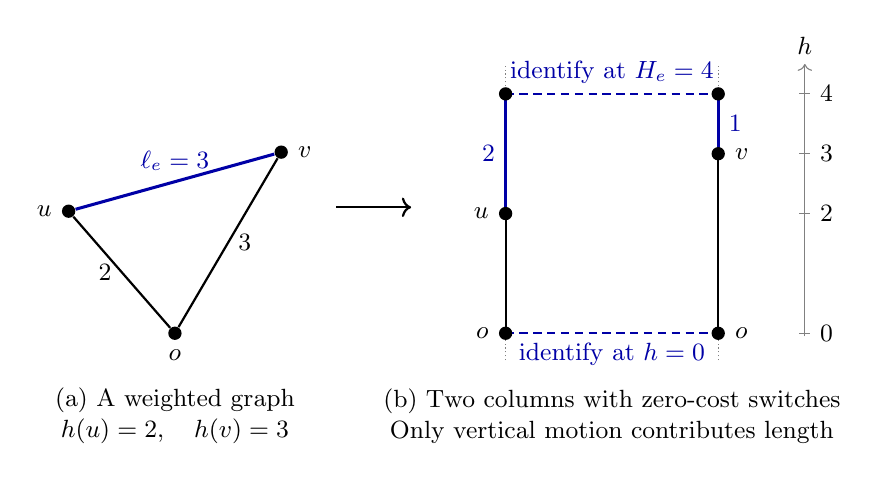
\begin{tikzpicture}[x=1cm,y=1cm,font=\small,
  vertex/.style={circle,fill=black,inner sep=1.7pt},
  twig/.style={blue!65!black,line width=1.1pt},
  identify/.style={blue!65!black,densely dashed,line width=.8pt}]
  \node[vertex,label=below:$o$] (o) at (0,0) {};
  \node[vertex,label=left:$u$] (u) at (-1.35,1.55) {};
  \node[vertex,label=right:$v$] (v) at (1.35,2.3) {};
  \draw[thick] (o)--node[left] {$2$} (u);
  \draw[thick] (o)--node[right] {$3$} (v);
  \draw[twig] (u)--node[above] {$\ell_e=3$} (v);
  \node[align=center] at (0,-1.05) {(a) A weighted graph\\$h(u)=2,\quad h(v)=3$};

  \draw[->,thick] (2.05,1.6)--(3,1.6);

  \begin{scope}[shift={(4.2,0)},y=.76cm]
    \draw[gray,densely dotted] (0,-.45)--(0,0);
    \draw[gray,densely dotted] (2.7,-.45)--(2.7,0);
    \draw[thick] (0,0)--(0,2);
    \draw[thick] (2.7,0)--(2.7,3);
    \draw[twig] (0,2)--node[left] {$2$} (0,4);
    \draw[twig] (2.7,3)--node[right] {$1$} (2.7,4);
    \draw[gray,densely dotted] (0,4)--(0,4.5);
    \draw[gray,densely dotted] (2.7,4)--(2.7,4.5);
    \draw[identify] (0,0)--node[below] {identify at $h=0$} (2.7,0);
    \draw[identify] (0,4)--node[above] {identify at $H_e=4$} (2.7,4);
    \node[vertex,label=left:$o$] at (0,0) {};
    \node[vertex,label=right:$o$] at (2.7,0) {};
    \node[vertex,label=left:$u$] at (0,2) {};
    \node[vertex,label=right:$v$] at (2.7,3) {};
    \node[vertex] at (0,4) {};
    \node[vertex] at (2.7,4) {};
    \draw[->,gray] (3.8,-.05)--(3.8,4.5) node[above,black] {$h$};
    \foreach \h in {0,2,3,4} {
      \draw[gray] (3.73,\h)--(3.87,\h) node[right,black] {$\h$};
    }
  \end{scope}
  \node[align=center] at (5.55,-1.05) {(b) Two columns with zero-cost switches\\Only vertical motion contributes length};
\end{tikzpicture}
\caption{An exact example of Proposition~\ref{geo:realization}.
The black edges form a shortest-path tree rooted at $o$.
The non-tree edge is replaced by two ascending twigs of lengths
$(\ell_e+h(v)-h(u))/2=2$ and $(\ell_e+h(u)-h(v))/2=1$.
Their tips have the same height $H_e=4$ and are identified.
Dashed horizontal segments denote identifications, not extra edges;
the dotted vertical tails do not shorten original distances.}
\label{fig:column-realization}
\end{figure}


\subsection{Consequences of the circular order}

The circular order gives separation statements used later for ordered
fields and the seed packing argument. These statements concern the column
graph, so they hold simultaneously for all height bands. Its outerplanarity
will also give the two-portal estimate in the next subsection.

\begin{lemma}[Chord separation]\label{geo:chord-separation}
Let $uv$ be an edge of a noncrossing circular graph.  Any graph path from
the strict interior of one circular $u$--$v$ arc to the strict interior of
the other visits $u$ or $v$.
\end{lemma}

\begin{proof}
A path avoiding $u,v$ and changing arcs has an edge whose endpoints lie
in the two strict interiors.  Its endpoints alternate with $u,v$, which
contradicts noncrossing.
\end{proof}

\begin{lemma}[Gaps of a connected set]\label{geo:gap}
Let $S$ be a nonempty connected vertex set in a noncrossing circular graph.
Every graph path avoiding $S$ lies in one of the open circular gaps between
consecutive vertices of $S$.  Here the complement of a singleton is regarded
as one gap.  Connectivity of $S$ and the path may be witnessed using
different subgraphs of the same noncrossing graph.
\end{lemma}

\begin{proof}
Suppose an edge $uv$ of the path joined distinct gaps.  Then each strict
circular $u$--$v$ arc contains a vertex of $S$.  A path inside $S$ joining
these two vertices would have to visit $u$ or $v$ by
Lemma~\ref{geo:chord-separation}.  Both endpoints lie outside $S$, a
contradiction.  Thus each edge stays in one gap, and so does the whole path.
\end{proof}

\begin{lemma}[Skipping a column]\label{geo:skipping}
Give an open circular arc its linear order, and assume its complementary
closed arc contains a column index.  Let a vertex walk stay in the open
arc, and let an index $i$ lie strictly between its initial and final indices.
Either the walk visits $i$, or one of its edges has endpoints strictly on
opposite sides of $i$.  In the latter case the edge is a non-neighbor link.
If a second path starts strictly between the endpoints of this edge and
leaves that strict interval, it visits an endpoint of the edge.
\end{lemma}

\begin{proof}
If the walk avoids $i$, take its first edge changing from one side of $i$
to the other.  The index $i$ lies on one strict circular arc between its
endpoints, and an index in the complementary closed arc lies on the other.
They are therefore not cyclic neighbors.  The final assertion is
Lemma~\ref{geo:chord-separation}.
\end{proof}

\begin{lemma}[Outerplanarity]\label{geo:outerplanar}
Every active graph $G_I$ is outerplanar and has no $K_{2,3}$ minor.
\end{lemma}

\begin{proof}
Place the indices on a circle and draw each edge as a straight chord.
The noncrossing condition makes this an outerplanar drawing.  Add a new
vertex in the complementary disk on the sphere and join it to every
column vertex by a disjoint radial star.  The resulting cone graph is
planar.  If $G_I$ had a $K_{2,3}$ minor, perform its deletions and contractions
while retaining the new vertex and one edge from it to every contracted
branch set.  The resulting planar minor contains the cone over $K_{2,3}$.
That cone contains $K_{3,3}$: add the cone vertex to the part of size two.
This is impossible, since a simple bipartite planar graph on six vertices
has at most eight edges, whereas $K_{3,3}$ has nine.
\end{proof}

\begin{lemma}[Connected distance sublevels]\label{geo:sublevel}
Fix a component of $X_I$, a source $o$ in it, and a height $H\in I$.
Put $q_i=d_I(o,(i,H))$, taking $q_i=+\infty$ outside that component.
For every real $t$, the nonempty set $\{i:q_i\le t\}$ is connected in
$G_I$.
\end{lemma}

\begin{proof}
For an index $i$ in the set, take a shortest path from $o$ to $(i,H)$.
If it visits a column $j$ at height $H'$, stop there and move vertically
to $(j,H)$.  The cost of this new ending is $|H-H'|$, at most the vertical
variation of the discarded suffix.  Thus $q_j\le q_i\le t$.  The projected
path therefore lies in the sublevel set and joins $i$ to the source column.
Taking these paths for all $i$ proves connectivity.  This argument also
shows that every source-column representative belongs to the sublevel
whenever the sublevel is nonempty.
\end{proof}

\subsection{Portals and radial cells}

We will cover the entrances to a connected radial superlevel set by at
most two controlled balls.  This estimate will then bound distances
within the connected pieces of each radial layer.

In this subsection $J$ is a closed band of width $a>0$, $H_*$ is its
midheight, and we work in a fixed component of $X_J$.  Choose a basepoint
$o$ and define
\[
 b_i=d_J(o,(i,H_*)).
\]
For a point $v=(i,H)$ in the band,
\begin{equation}\label{geo:radial-estimates}
 \bigl|d_J(o,v)-b_i\bigr|\le a/2,
 \qquad |b_i-b_j|\le a\quad\text{if }ij\in G_J.
\end{equation}
The second estimate follows by traveling from the two midpoints to an
available switch, at cost at most $a$.  We occasionally use the weaker
bound $2a$ without further comment.

\begin{lemma}[Two portals]\label{geo:portals}
Let $C$ be a component of the subgraph of $G_J$ induced by $\{i:b_i\ge t\}$.
An \emph{entrance column} of $C$ is an index in $C$ adjacent to an index
with radial value below $t$.  If entrance columns exist, there are at most
two of their midpoints, called portals, such that every point on every
entrance column lies within $200a$ in $d_J$ of one of the portals.
Every portal has radial value in $[t,t+a)$.  If $t>a/2$ and $C$ is nonempty,
entrance columns exist.
\end{lemma}

\begin{proof}
An entrance column has $t\le b_i<t+a$ by
\eqref{geo:radial-estimates}.  When $t<30a$, all entrance midpoints have
distance less than $31a$ from $o$.  Any one is therefore within $62a$ of
every other, and within $63a$ of every point on every entrance column.
One portal suffices in this case.

Suppose $t\ge30a$.  Let $L$ be the projection to columns of the closed
ball $B_{d_J}(o,t-12a)$.  Shortest paths from $o$ to the points
of the ball stay in the ball, so $L$ is connected.  Every $j\in L$ has
$b_j\le t-12a+a/2$, and hence $L$ is disjoint from $C$.

Assume there are three entrance midpoints $x_1,x_2,x_3$ at pairwise
distance greater than $100a$.  Starting from each $x_k$, follow a shortest
path toward $o$ until its first visit to a column of $L$.  This portion
has length at most $13a$: by that length it reaches a point at radial
distance $t-12a$.  Its projection joins $C$ to $L$.  The three projected
portions are vertex-disjoint.  Indeed a common column would permit a
vertical transfer of length at most $a$, giving a path of length at most
$13a+a+13a<100a$ between the corresponding entrance points.

For each portion retain the segment after its last visit to $C$ and
before its first visit to $L$.  Its interior avoids both sets.  It has
an internal vertex, since its endpoints have radial values differing by
at least $12a-a/2>a$, while adjacent columns differ by at most $a$.
Contract the connected sets $C$ and $L$, and contract each of the three
nonempty connector interiors to a separate vertex.  This gives a
$K_{2,3}$ minor, contrary to Lemma~\ref{geo:outerplanar}.

A maximal set of entrance midpoints at mutual distances greater than
$100a$ thus has cardinality at most two.  Maximality covers every entrance
midpoint within $100a$, and the extra vertical distance is at most $a/2$.
This proves the stated $200a$ bound.  Finally a representative of $o$ has
radial value at most $a/2$.  If $t>a/2$, any nonempty high component is a
proper subset of the connected graph and has an entrance.
\end{proof}

\begin{figure}[tbp]
\centering
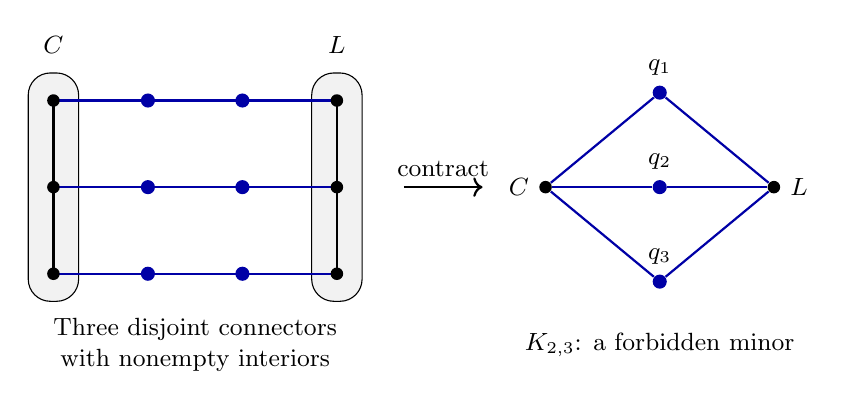
\begin{tikzpicture}[x=1cm,y=1cm,font=\small,
  vertex/.style={circle,fill=black,inner sep=1.6pt},
  interior/.style={circle,fill=blue!65!black,inner sep=1.8pt}]
  \draw[fill=gray!10,rounded corners=8pt] (-.32,-1.45) rectangle (.32,1.45);
  \draw[fill=gray!10,rounded corners=8pt] (3.28,-1.45) rectangle (3.92,1.45);
  \draw[thick] (0,-1.1)--(0,1.1);
  \draw[thick] (3.6,-1.1)--(3.6,1.1);
  \foreach \y in {-1.1,0,1.1} {
    \draw[blue!65!black,thick] (0,\y)--(3.6,\y);
    \node[vertex] at (0,\y) {};
    \node[vertex] at (3.6,\y) {};
    \node[interior] at (1.2,\y) {};
    \node[interior] at (2.4,\y) {};
  }
  \node at (0,1.8) {$C$};
  \node at (3.6,1.8) {$L$};
  \node[align=center] at (1.8,-2) {Three disjoint connectors\\with nonempty interiors};
  \draw[->,thick] (4.45,0)--(5.45,0) node[midway,above] {contract};

  \node[vertex,label=left:$C$] (C) at (6.25,0) {};
  \node[vertex,label=right:$L$] (L) at (9.15,0) {};
  \foreach \y/\k in {1.2/1,0/2,-1.2/3} {
    \node[interior,label=above:$q_\k$] (q\k) at (7.7,\y) {};
    \draw[blue!65!black,thick] (C)--(q\k)--(L);
  }
  \node at (7.7,-2) {$K_{2,3}$: a forbidden minor};
\end{tikzpicture}
\caption{The hypothetical obstruction in Lemma~\ref{geo:portals}.
Three sufficiently separated entrance points would give vertex-disjoint
paths from the connected high set $C$ to the connected low set $L$.
After trimming, each connector has a nonempty interior avoiding both
sets. Contracting $C$, $L$, and the three interiors gives $K_{2,3}$,
which cannot be a minor of the outerplanar column graph.
The drawing records this contraction; it is not an outerplanar drawing
of a configuration that the column model permits.}
\label{fig:two-portals}
\end{figure}


\begin{definition}[Radial cells]\label{geo:cell-definition}
Fix $D>0$ and an offset $\theta\in[0,D)$.  Partition the indices into
layers by assigning $i$ to the unique half-open interval
\[
 [\theta+nD,\theta+(n+1)D),\qquad n\in\mathbb Z,
\]
containing $b_i$.  Split each layer into the connected components of its
induced subgraph of $G_J$.  A \emph{cell} is the image in $X_J$ of all
intervals $\{i\}\times J$ belonging to one such component. Its
\emph{frontier} $\partial C$ is the union of their images for indices
adjacent in $G_J$ to an index outside the cell.
\end{definition}

This is a partition of the column indices, not necessarily a disjoint
partition of their quotient images.  If two cells share a quotient point,
that point belongs to the frontier of each: a switch chain identifying
representatives in the two cells has a first edge leaving either cell.
Consequently formulas that agree with the unchanged data on all frontiers
give unambiguous values at such shared points.

Here a \emph{weak diameter} bound measures distances in the whole band;
the paths witnessing those distances may leave the cell.

\begin{lemma}[Diameter of cells]\label{geo:cells}
Assume $a\le D/1000$.  Every radial cell is compact and path-connected,
and has weak diameter at most $10D$ in $d_J$.  Its frontier is compact,
possibly empty.
\end{lemma}

\begin{proof}
Each cell is the image of finitely many closed column intervals.  Its
column graph is connected, which makes that image path-connected.  The
same finite-union argument proves compactness of the cell and frontier.

Let $q$ be the lower threshold of its layer.  If $q\le30a$, every point
of the cell has distance less than $D+31a$ from $o$, so the diameter bound
follows.  Suppose $q>30a$ and let $C^+$ be the component of $\{b_i\ge q\}$
containing the cell.  It has at most two entrance portals by
Lemma~\ref{geo:portals}.

Take $v$ in the cell and follow a shortest path to $o$ until the first
switch below threshold $q$.  Before that switch the projected path stays
in $C^+$: two adjacent high columns belong to the same high component.
The last high column is an entrance, and the switch point has radial
distance at least $q-a/2$.  Since $d_J(o,v)<q+D+a/2$, the portion from $v$
to that point has length less than $D+a$.  Some portal is within $200a$
of that point.  Thus the cell is contained in the union of two closed
balls of radius $D+210a$ around its portals.

A connected set contained in the union of two closed balls either lies
in one of them or meets their intersection.  To see the second alternative
when neither ball contains the set, intersect both balls with the connected
set; two nonempty disjoint closed subsets could not cover it.  In that
case the centers have distance at most $2(D+210a)$.  In either alternative
the cell has diameter at most $4(D+210a)<10D$.
\end{proof}

\begin{lemma}[Padding and separation of cell interiors]\label{geo:padding}
Let $v=(i,H)\in X_J$, and let $T=\theta+D\mathbb Z$ be the radial
threshold set.  If
\begin{equation}\label{geo:padding-condition}
 \dist(b_i,T)>\rho+2a,
\end{equation}
then every point reachable from $v$ by a band path of length at most
$\rho$ has all its representatives in the same cell as $i$.  Moreover
$d_J(v,\partial C)>\rho$ for that cell.

For uniform $\theta\in[0,D)$, the probability that
\eqref{geo:padding-condition} fails is at most
\[
 \min\{1,\,2(\rho+2a)/D\}.
\]
There is no factor for the number of representatives of $v$: their
radial values differ pairwise by at most $a$.

In particular, if $a\le D/1000$ and the radial values of two points are
at distance greater than $0.02D$ from the thresholds, then their distances
to their respective frontiers are greater than $0.01D$.  If they belong
to different cells, their mutual $d_J$-distance is greater than $0.01D$.
\end{lemma}

\begin{proof}
If a band path from $v$ of length at most $\rho$ visits column $k$, join
its visit point to $(k,H_*)$ and join $v$ to $(i,H_*)$.  The triangle
inequality gives
\[
 |b_k-b_i|\le\rho+a.
\]
Thus every visited column stays in $i$'s layer under
\eqref{geo:padding-condition}; its projected path puts it in the same
connected component of that layer.  The same argument applies after any
zero-cost switch chain at an endpoint, proving the assertion about all
representatives.

Every frontier column has its radial value within $a$ of one of the
cell's layer thresholds: its neighbor outside the cell cannot belong
to the same layer.  If $z$ lies on a frontier column $k$, then
\[
 d_J(v,z)\ge |b_i-b_k|-a
       \ge \dist(b_i,T)-2a>\rho.
\]
The formula remains true for an empty frontier with distance $+\infty$.
The offset estimate is the length, at most $2(\rho+2a)$, excluded in one
period.  Two representatives at height $H$ have midpoint distance at
most $2|H-H_*|\le a$, since their points at height $H$ are identical.
This proves the representative assertion without a union bound.

For the numerical conclusion use
$0.02D-2a\ge0.018D>0.01D$.  A path to a different cell must first visit
a frontier column of the initial cell, so the same lower bound applies
to its length.
\end{proof}

The cell estimates will control the regions where the local updates act.
For interpolation we also need the entrance estimate at successive radial
thresholds. The resulting components form a rooted tree, with controlled
distances between the portals at successive levels.

\begin{lemma}[Successive portal levels]\label{geo:portal-levels}
Fix a step $\delta>1000a$.  At depth $n\ge1$ take the components of
$\{b_i\ge n\delta\}$ and give each its entrance portals from
Lemma~\ref{geo:portals}.  The depth-zero node is the whole component,
with its sole portal $o$.  Each positive-depth node has a unique parent.
For a node at depth $n$, every point on one of its columns with
$b_i<(n+1)\delta$, and every portal of one of its children, is within
$\delta+220a$ of one of its own portals.  Each child portal is at distance
at least $\delta-10a$ from every own portal.
\end{lemma}

\begin{proof}
A connected component at a higher threshold is contained in a unique
component at the preceding threshold, proving the parent assertion.
For $n\ge1$, repeat the root-geodesic argument in
Lemma~\ref{geo:cells} at lower threshold $n\delta$.  A point of the
node's own layer has radial distance below $(n+1)\delta+a/2$.  A child
portal has radial distance in
$[(n+1)\delta,(n+1)\delta+a)$.  In either case its geodesic reaches an
entrance of the parent node after length at most $\delta+2a$, and an
own portal is within a further $200a$.  The asserted upper bound follows.

An own portal has radial distance in $[n\delta,n\delta+a)$, whereas a
child portal has radial distance at least $(n+1)\delta$.  Their distance
is therefore at least $\delta-a$.  At depth zero the upper bounds follow
directly by taking $o$, and a depth-one portal is at distance at least
$\delta$ from it.  These estimates imply the stated bounds in every case.
\end{proof}

\section{Threshold sets and local coordinates}
\label{sets:section}

We construct cuts by assigning a measurable set of labels to every point
of the column model. Along a column these sets will grow with height,
with symmetric-difference measure equal to the vertical length. At a
switch the sets will agree exactly. Every resulting cut distance is
therefore bounded by the length of every column path. The local updates
must produce lower separation while preserving these two properties.

There are two systems, called $A$ and $B$. System $A$ also uses the
connected components of a label's active columns to separate points.
System $B$ supplies a second local separation test. Evolving distributions
of monotone cuts through smaller scales is a central mechanism in
Sidiropoulos's nonpositively curved planar construction~\cite[Sections~4--5]{Sidiropoulos13}.
Here the updates must also preserve the exact sets where local formulas meet.

\subsection{Charts on a fixed label space}

For each system fix a label space
\[
 (\Omega,\mu)=\bigl(\R\times\{-1,1\}^{\N},
                   \mathcal L\otimes\nu\bigr),
\]
where $\mathcal L$ is Lebesgue measure and $\nu$ is the product of fair sign
measures. Every set in that system is a subset of this same $\Omega$.
The random choices of updates are independent of the label coordinates;
we condition on those choices when describing the sets.

A \emph{chart} consists of a region $\mathcal R\subset X$, a height band
$I$ containing its heights, a field $P$ on the corresponding component of
$X_I$ (or on all of $X_I$), and measurable functions
$Z:\Omega\to\R$ and $\sigma:\Omega\to\{-1,1\}$ whose joint pushforward
measure is Lebesgue measure times a fair sign. For $v\in\mathcal R$ set
\begin{equation}\label{sets:formula}
 \mathcal A_v=\{\omega\in\Omega:
 Z(\omega)<h(v)+\sigma(\omega)\kappa P(v)\}.
\end{equation}
Write $\mathcal B_v$ for system $B$. The positive constant $\kappa$ is
fixed separately in each system; its values $\kappa_A,\kappa_B$ will be
chosen in Section~\ref{sets:parameters}.

At each stage there are finitely many chart identifiers. Each identifies
common field and label data and their current region. These regions
partition $X$, with a fixed rule for ties. A region may be disconnected;
its connected pieces do not receive different identifiers. When some
points receive a new chart, the old identifier is retained on the
remaining region. Initially each system has one chart on $X$, with
$P=0$, $Z$ the original Lebesgue coordinate, and $\sigma$ the first sign
coordinate.

Write $\Lip_{\mathrm{vert}}(P)$ for the supremum of the Lipschitz constants
of $P$ on its vertical column intervals. The following identity explains
both the upper invariant and the purpose of changing the field.

\begin{lemma}[Vertical control and rebasing]\label{sets:vertical}
For two points whose sets are expressed in common chart variables,
\begin{equation}\label{sets:distance}
 \mu(\mathcal A_v\mathbin\triangle\mathcal A_w)
   =\max\{|h(v)-h(w)|,\kappa|P(v)-P(w)|\}.
\end{equation}
If $\kappa\Lip_{\mathrm{vert}}(P)<1$ and $P$ respects switches, the sets are
nested increasingly on each column interval in the chart. Their
symmetric-difference measure there equals the vertical length.

A branch $P(v)=\psi(h(v))$, where $\psi:\R\to\R$ is Lipschitz with
$\kappa\Lip(\psi)<1$, can be represented by a fresh constant chart without
changing any sets.
\end{lemma}
\begin{proof}
For each sign, the symmetric difference of the two half-lines has measure
$|\Delta h+\sigma\kappa\Delta P|$. Averaging the signs gives
\eqref{sets:distance}. The functions $H\mapsto H\pm\kappa P(i,H)$
are increasing, and their average increment is the height increment.

For rebasing put $\phi_\sigma(H)=H+\sigma\kappa\psi(H)$.
These are increasing bijections of $\R$. Define the new coordinate on the
same label space by $Z'(\omega)=\phi_{\sigma(\omega)}^{-1}(Z(\omega))$.
Its pushforward measure is Lebesgue measure, since for $a<b$,
\[
 \mu\{a<Z'<b\}
 =\frac{\phi_+(b)-\phi_+(a)+\phi_-(b)-\phi_-(a)}2=b-a.
\]
Choose a sign coordinate unused anywhere earlier in this execution. It
is independent of $Z'$. Thus $(Z',\sigma')$ has the required joint
pushforward, and, for every label,
\[
 \{Z<\phi_\sigma(h)\}=\{Z'<h\}.
\]
This describes exactly the same sets by a chart with field zero.
\end{proof}

In an \emph{ordinary chart}, the field has the form
$P=c+\eta s$, where $\eta\in\{-1,1\}$ and either
$s(v)=d_I(o,v)$ for a fixed source $o$, or $s=0$.
For a constant field take $c=P$ and $\eta=1$.
Updating in \emph{ordinary orientation} means changing $s$ and converting
back using the same $c$ and $\eta$. System $A$ always uses ordinary charts.
System $B$ begins with an ordinary chart and later uses the additional
field type constructed in Section~\ref{ord:section}. Every recorded
$B$-field will have Lipschitz constant less than $5$ for finite $d_I$.

The interpolation in Section~\ref{int:section} will produce formulas for
ordinary charts. These formulas carry names: when the same formula is inherited
across an interpolation boundary, its name is preserved. When an interpolation formula becomes a chart, its new identifier
records the old chart, the particular interpolation, and the selected
formula's name, and retains the old label functions. Different old charts are not merged merely
because their formulas agree. Within one old chart, recording an inherited
formula therefore does not split a region merely because an internal
interpolation boundary was crossed.

\subsection{Exact gluing and component refinement}

Every local update is first expressed in the old chart variables. A
clipping replaces the old comparison field by its maximum with a proposal,
which is the minimum of finitely many fields. Several proposals are
combined by a finite maximum. On the boundary of each proposal's
domain the proposal lies below the old field, with a strict margin in
the spatial constructions below. Thus the clipping equals the old field
at the endpoints of every updated column interval and at any switch
leading outside the domain. Inside the domain all branches respect
switches and have vertical Lipschitz constants whose products with
$\kappa$ are less than one.

The new sets consequently retain the global upper invariant. For points
in one updated interval this follows from Lemma~\ref{sets:vertical}. For
points in different updated intervals, compare the first point with its
interval endpoint, then use the old nested sets between the two interval
endpoints, and finally compare with the second point. These three
comparisons preserve nesting, and their symmetric-difference measures
sum to the full vertical length. Unchanged points are handled by the
same comparison. This argument does not require a finite number of
updated intervals. Exact agreement at the boundary also preserves the
sets at every switching identification. A Lipschitz perturbation that
vanishes at the domain boundary admits the same interval-endpoint
argument, provided the updated field respects switches and still has
$\kappa\Lip_{\mathrm{vert}}(P)<1$. The later increments in system $B$
will satisfy these conditions.

Only after making the update do we record its winning formulas as new
charts. A spatial branch inherits the old label functions $Z,\sigma$;
a height-only branch is rebased as in Lemma~\ref{sets:vertical}. An
unchanged point keeps its old identifier. Height branches can have larger
slopes than the recorded ordinary or $B$-fields; after rebasing their
recorded fields are zero. Recording or rebasing these charts does not further change the newly
assigned subsets of $\Omega$. The identity \eqref{sets:distance} applies when the sets under
comparison are written in common label variables; the global nesting
and vertical-length invariant applies across all charts.

For a fixed label $\omega$, call a point \emph{active} when its assigned
set contains $\omega$. The active points of any column form an upper
interval. Besides membership, we can use the connected components joined
by active switches.

\begin{lemma}[Component refinement]\label{sets:component-refinement}
Suppose a system of sets is nested increasingly on each column, respects
switches, and has symmetric-difference measure at most vertical length.
It defines an $L_1$ pseudometric dominated by $d$. It also admits the
following refinement with the same upper bound.

For a label $\omega$, join two columns when one of their switches occurs
at a height active for $\omega$. To an active point assign the unit vector
indexed by its component in this finite graph, and to an inactive point
assign zero. Integrating the $\ell_1$ distances of these vectors gives the
refined pseudometric. It dominates the original symmetric-difference
pseudometric.

If a non-neighbor link has inactive tip and two active points have
representatives strictly on opposite sides of it, their refined distance
for that label is $2$.
\end{lemma}
\begin{proof}
For a fixed label all active points of a column have the same component
coordinate. On a vertical segment the vector changes only when activity
changes, and its $\ell_1$ cost is the original indicator cost. At an active
switch the two columns belong to the same component; at an inactive switch
both vectors are zero. Integration and any finite path give the upper
bound. A membership difference always costs one, proving domination.

Every switch incident to an endpoint column of a non-neighbor link is at
or below its tip. If the tip is inactive, nesting makes all such switches
inactive. A path of column indices between the two strict sides must pass
through an endpoint of the link, by noncrossing. No active path can do so.
The active points therefore have different unit coordinates.

There are only finitely many possible components, which can be indexed by
subsets of the columns. An active link can be tested at its maximum
switching height, so all coordinates are measurable. Subtracting the vector
assigned to one fixed reference point makes each assignment integrable:
the integrated norm of the difference is bounded by the distance to that
point. The same subtraction works for the unrefined indicator system.
\end{proof}

Only system $A$ will be refined, once, after the last scale. We therefore
track changes of membership during the construction, without tracking
changes of component coordinates. The final component separation will
be certified by activity at two vertices and inactivity at one fixed tip.

\subsection{The estimates required of a local update}

An update at scale $r>0$ will try to separate original vertex pairs
whose distances lie in $[r,2r)$. At scale $r$, a pair $(x,y)$ is
\emph{eligible} if the two closed balls $B_d(x,5r)$ and $B_d(y,5r)$
lie in one common old chart region in system $A$ and in one common
old chart region in system $B$. The common region may differ between
the two systems. This condition supplies common field and label data
for all short paths used in the pair's local tests.

The construction below will give constants $M,C_0<\infty$ and
$b,p,\rho_0>0$, independent of the graph and the update history,
with three properties.
\begin{enumerate}
\item At every point of the full column space $X$, an update at scale
$r$ changes each unrefined label set by symmetric-difference measure
at most $Mr$.
\item For a vertex pair with $d(x,y)\in[r,2r)$, conditional on any past
in which $(x,y)$ is eligible, the update
has probability at least $p$ of producing either unrefined symmetric-difference separation
at least $br$ in one system, or a non-neighbor link separating
representatives of $x,y$ strictly and a system-$A$ label set of measure
at least $br$ on which $x,y$ are active and the link's tip is inactive.
\item Suppose a fixed ball $B_d(v,\rho r)$ lies in one old chart region in each
system, where $0<\rho\le\rho_0$. Conditional on the past, the probability
that this ball meets different new chart regions in either system is
at most $C_0(\rho+\eta_0)$.
\end{enumerate}
Here $\eta_0$ is a dimensionless upper bound for the relative mesh of
the finite grids used to sample update parameters. It can be chosen
arbitrarily small after the finite set of scales is fixed; the
sampling convention is given in Section~\ref{sets:setup}.

Propositions~\ref{pad:success} and~\ref{pad:persistence} establish
these estimates after the local construction is complete. The third
estimate keeps a pair eligible until its own scale with positive
probability. The first then prevents sufficiently smaller scales from
erasing the second estimate's gain. For a component certificate, this
requires movement control at the tip as well as at the two vertices;
that is why the first estimate concerns all of $X$. Section~\ref{pad:assembly}
combines the estimates by using schedules whose successive scales
differ by a sufficiently large fixed factor.

\section{Interpolation by single-source distance functions}
\label{int:section}

All distances in this section are intrinsic to one connected component
$Y$ of a closed band $X_J$.  We write $d_J$ for this distance.  The width
of $J$ is denoted by $a$, and its midpoint by $H_*$.  The active column
graph and its radial coordinate $b_i=d_J(o,(i,H_*))$ are as in
Section~\ref{geo:section}; we choose $o$ at height $H_*$.  The choices of
$o$ and of all portals below are made before any random parameters in
this section are sampled.

The construction will repeatedly use signed point-distance formulas as
local data. We therefore approximate a function of Lipschitz constant
strictly below one by formulas $c\pm d_J(k,\cdot)$, while controlling where the
selected formula changes. Each formula has a fixed source and sign, a
random additive constant, and a name. When the construction reuses a
formula, it retains that name. Stability on a small ball means that one
name is selected throughout the ball, not merely that the values agree
at the interfaces.

\begin{theorem}[Thin-band interpolation]\label{int:interpolation}
Let $0<\zeta<1$, let $E>0$, and set
\begin{equation}\label{int:constants}
 \begin{gathered}
 \delta=E/8,\qquad a_0=10^{-6}\zeta\delta,\qquad
 q=\zeta\delta/20,\\
 \rho_0=\zeta\delta/1000,\qquad
 M=\lceil15/\zeta\rceil+3,\qquad N=6(M+1).
 \end{gathered}
\end{equation}
Suppose $0<a\le a_0$, and let $p:Y\to\R$ be
$(1-\zeta)$-Lipschitz for $d_J$.  There is a random function
$Q:Y\to\R$, obtained using finitely many independent scalar noises
uniform on $[q,2q]$, with the following properties.
\begin{enumerate}
\item For every realization, $Q$ respects all switches, is
$1$-Lipschitz for $d_J$, and satisfies $|Q(v)-p(v)|\le6\delta<E$.
\item Its pieces use finitely many named atoms of the form
\begin{equation}\label{int:atom-form}
 A(v)=C+\varepsilon d_J(k,v),\qquad \varepsilon\in\{-1,1\},\quad k\in Y.
\end{equation}
Each name specifies a source $k$ and sign $\varepsilon$ fixed before the
noises are sampled; the intercept $C$ is random. Whenever the construction
reuses an atom, it retains its name.
\item For a fixed $x\in Y$ and $0<\rho\le\rho_0$, there is a list
$\mathcal A(x,\rho)$ of at most $N$ atom names and sources, determined
without the noises, that contains the name of every atom selected by $Q$ on
$B_{d_J}(x,\rho)$.  Except on an event of probability at most
\begin{equation}\label{int:probability}
 \frac{N^2}{q}(8\rho+\eta),
\end{equation}
one named atom is selected throughout this ball.
\end{enumerate}
Here $\eta=0$ for continuous uniform noises.  Alternatively, each noise
may be uniform on an equally spaced grid including both endpoints of
$[q,2q]$, and $\eta$ in \eqref{int:probability} may be the largest grid
spacing.  The same conclusions hold for any set of points reached
from $x$ by band paths of length at most $\rho$, including the points
and representatives encountered on those paths.
\end{theorem}

\subsection{The tree of superlevel components}

For every integer $n\ge0$, take the connected components of the
subgraph on columns with $b_i\ge n\delta$.  Its nonempty components
are called nodes of depth $n$.  The sole node of depth zero is the
root.  A node of depth $n+1$ is contained in exactly one node of depth
$n$, its parent.  Because there are finitely many columns and all
$b_i$ are finite, there are only finitely many nodes.  The layer
belonging to a node $\nu$ of depth $n$ consists of the full columns in
that node satisfying
\[
 n\delta\le b_i<(n+1)\delta.
\]
A node can have an empty layer; it is still retained in the tree.
Every column has exactly one layer node.

The layers specify where a node's formula will be used.  The formula itself
will be defined on all of $Y$.  Near an entrance to a child node, the child
and parent formulas will agree exactly; this will allow us to paste their
restrictions across layer boundaries without changing values or names.

For a positive-depth node, choose its set $K_\nu$ of one or two
entrance portals using Lemma~\ref{geo:portals}.  The portals are
midheight points on entrance columns.  At the root set $K_\nu=\{o\}$.
The radial and portal estimates of Lemma~\ref{geo:portal-levels} give
the following facts, which also apply to the root with this convention:
\begin{align}
 \min_{k\in K_\nu}d_J(k,v)&\le\delta+220a
 &&\text{if $v$ is in the layer of $\nu$ or is a child portal},
 \label{int:near-portal}\\
 d_J(k,v)&\ge\delta-10a
 &&\text{if $k\in K_\nu$ and $v$ is a child portal}.
 \label{int:separated-portals}
\end{align}
For a positive-depth node of depth $n$, every $k\in K_\nu$ also
satisfies
\begin{equation}\label{int:portal-radial}
 n\delta\le d_J(o,k)\le n\delta+2a.
\end{equation}
Every point on an entrance column is within $200a$ of $K_\nu$.
These are statements about $d_J$, so paths witnessing them may leave
the corresponding node.

\subsection{The formulas and their deterministic estimates}

At each node we first approximate the input by positive distance cones
based at its portals. We then constrain this tentative formula so that
it agrees with the parent near every entrance. The strict Lipschitz
bound on the input will limit how many generations an accurate atom
can be inherited through.

For every portal $k\in K_\nu$, sample an independent noise
$\alpha_{\nu k}\in[q,2q]$. At every nonroot node also sample
$\alpha'_{\nu k},\alpha''_{\nu k}\in[q,2q]$. All these noises are
mutually independent. Define formulas on the whole of $Y$, recursively
down the tree. The tentative formula is
\[
 T_\nu(v)=\min_{k\in K_\nu}
       \bigl(p(k)+d_J(k,v)+\alpha_{\nu k}\bigr).
\]
At the root put $F_\nu=T_\nu$. This is $1$-Lipschitz, because
distance functions and their finite minima are $1$-Lipschitz.

Now let $\nu$ have parent $\pi$, whose formula is already defined
and $1$-Lipschitz. To preserve the parent at the interfaces, we will
constrain $T_\nu(v)$ to an interval containing $F_\pi(v)$ that
collapses to this single value near $K_\nu$. Define two envelopes
of cones based at the parent values:
\begin{align*}
 A_\nu(v)&=\min_{k\in K_\nu}
     \bigl(F_\pi(k)+d_J(k,v)-\alpha'_{\nu k}\bigr),\\
 B_\nu(v)&=\max_{k\in K_\nu}
     \bigl(F_\pi(k)-d_J(k,v)+\alpha''_{\nu k}\bigr).
\end{align*}
If $d_J(k,v)<q/2$ for a portal $k$, the term with source $k$
in the first envelope is below $F_\pi(v)$, and its term in the
second is above $F_\pi(v)$. Indeed the parent changes by at most
$d_J(k,v)$, whereas each noise is at least $q$.
Thus $A_\nu(v)<F_\pi(v)<B_\nu(v)$ near every portal, even if
the other portal's cones have different values. The desired interval is
\[
 [L_\nu(v),U_\nu(v)]
 =\bigl[\min(F_\pi(v),B_\nu(v)),
        \max(F_\pi(v),A_\nu(v))\bigr].
\]
It always contains the parent value and reduces to that value in
these portal neighborhoods. Clamp the tentative formula to this interval:
\[
 F_\nu(v)=\min\bigl(U_\nu(v),\max(L_\nu(v),T_\nu(v))\bigr).
\]
All the formulas remain $1$-Lipschitz on $Y$, since finite minima and
maxima preserve this property. This completes the recursive construction.

The new atoms of a nonroot node are
\begin{align}
 p(k)+d_J(k,v)+\alpha_{\nu k},\qquad
 F_\pi(k)+d_J(k,v)-\alpha'_{\nu k},\qquad
 F_\pi(k)-d_J(k,v)+\alpha''_{\nu k}.
 \label{int:three-types}
\end{align}
The root has its single tentative atom. An intercept $F_\pi(k)$ in
\eqref{int:three-types} is a scalar, not an instruction to inherit the
atom selected at $k$. Each expression in \eqref{int:three-types} is a
new atom with source $k$. In contrast, selecting the branch
$F_\pi(v)$ inherits its atom and its name.

Fix a total priority order on names in which all smaller-depth names
precede larger-depth names. In every minimum or maximum, resolve
equal values in favor of the earliest name. Multiple appearances of
one inherited atom have the same name. This completely specifies a
named atom selected by every formula at every point.

\begin{lemma}[Accuracy and equality collars]\label{int:deterministic}
Every node formula $F_\nu$ has error at most $5\delta$ at every portal
of a child of $\nu$, and error at most $6\delta$ on its own layer.
At a nonroot node with parent $\pi$, if
\[
 \dist_{d_J}(v,K_\nu)\le c_0:=\zeta\delta/50,
\]
then $F_\nu(v)=F_\pi(v)$, with the same selected atom name.
\end{lemma}

\begin{proof}
Since $c_0<q/2$, the portal-neighborhood calculation above gives
$U_\nu(v)=L_\nu(v)=F_\pi(v)$ in the stated collar. The priority
convention retains the parent atom even if $T_\nu(v)=F_\pi(v)$.

For accuracy, the Lipschitz bound of $p$ gives, at every point,
\begin{equation}\label{int:tentative-bounds}
 p(v)+\zeta\dist_{d_J}(v,K_\nu)+q
 \le T_\nu(v)
 \le p(v)+(2-\zeta)\dist_{d_J}(v,K_\nu)+2q.
\end{equation}
In the situations of \eqref{int:near-portal}, its upper bound is
less than $p(v)+3\delta$, by \eqref{int:constants}.  This proves both
accuracy assertions at the root.

Proceed by induction.  At a nonroot node, the inductive hypothesis
gives $|F_\pi(k)-p(k)|\le5\delta$ for all its own portals.  Therefore,
writing $r_\nu(v)=\dist_{d_J}(v,K_\nu)$,
\begin{align}
 A_\nu(v)&\ge p(v)-5\delta+\zeta r_\nu(v)-2q,
 \label{int:upper-atom-bound}\\
 B_\nu(v)&\le p(v)+5\delta-\zeta r_\nu(v)+2q.
 \label{int:lower-atom-bound}
\end{align}
At a child portal, \eqref{int:separated-portals} and
$a\le10^{-6}\zeta\delta$ imply
$\zeta r_\nu(v)\ge2q$.  Hence
$U_\nu(v)\ge p(v)-5\delta$ and
$L_\nu(v)\le p(v)+5\delta$.  Clamping a number in
$[p(v),p(v)+3\delta]$ to an interval with these two properties gives
a value in $[p(v)-5\delta,p(v)+5\delta]$.

On the own layer, the same argument without the favorable distance
term gives $U_\nu(v)\ge p(v)-5\delta-2q$ and
$L_\nu(v)\le p(v)+5\delta+2q$.  Since $2q\le\delta/10$, the
clamped value has error at most $5.1\delta<6\delta$.
\end{proof}

Define $Q$ on a representative $(i,H)$ by the formula of the unique
layer node of column $i$.  Two columns joined by a switch have radial
values differing by at most $2a<\delta$, so their layer depths are
equal or consecutive.  At equal depths their nodes coincide.  At
consecutive depths the upper node is a child of the lower node, and
the upper column is an entrance column.  Its switch point is within
$200a<c_0$ of an upper portal, so Lemma~\ref{int:deterministic} gives
the same value and atom name from both representatives.  Applying this
to every switch also gives consistency under transitive identifications.
Thus $Q$ is defined on $Y$.  It is $1$-Lipschitz on each column and
respects switches; summing along band paths shows that it is
$1$-Lipschitz for $d_J$.  Its accuracy follows from
Lemma~\ref{int:deterministic}.

\subsection{One deterministic ancestor chain for a small ball}

The pasted function is now well defined and has the required approximation
error.  To control changes of its selected formula, we next show that a
small ball sees one node formula and only boundedly many of its ancestors.
This step uses the geometry and the strict Lipschitz bound of the input;
the random comparison estimate comes afterward.

\begin{lemma}\label{int:common-formula}
For $x\in Y$ and $0<\rho\le\rho_0$, one node $\nu$, determined
without the interpolation noises, satisfies $Q=F_\nu$ on
$B_{d_J}(x,\rho)$, including equality of selected atom names.
If $n$ is the depth of $\nu$, every point of this ball has a
representative on a column with $b_i\ge n\delta$.
\end{lemma}

\begin{proof}
The closed ball is connected by geodesics through its center.  Include
all representatives of all its points in its column projection.  For
any two such representatives their radial values differ by at most
$2\rho+2a<\delta$, using the radial comparison with $d_J(o,\cdot)$.
Thus their layer depths take either a single value or two consecutive
values $n,n+1$.  The projected graph is connected, and all its columns
have $b_i\ge n\delta$.  They therefore belong to one superlevel node
$\nu$ at depth $n$.  In the single-depth case this proves the result.

Otherwise choose a represented point of layer depth $n$ in the ball.
For any represented point $v$ of depth $n+1$, concatenate its geodesic
to the center with a geodesic to the chosen point.  This is a band
path of length at most $2\rho$.  Its last crossing from depth $n$
to depth $n+1$, when traversed toward $v$, enters the child node
containing the representative of $v$.  The entry column is an entrance
column of that child.  Hence $v$ is within
$2\rho+200a<c_0$ of a portal of that child.  The equality collar of
Lemma~\ref{int:deterministic} identifies its formula and its selected
atom with those of $\nu$ at $v$.  This proves the assertion for every
representative.  All the choices in this argument depend only on the
band geometry and the ball.
\end{proof}

\begin{lemma}[Bounded depth of a selected atom]\label{int:depth}
For the node $\nu$ supplied by Lemma~\ref{int:common-formula}, every
atom selected by $F_\nu$ on the ball originates in $\nu$ or one of
its last $M$ ancestors.  Consequently at most $N$ atom names can be
selected there.
\end{lemma}

\begin{proof}
We first prove an obstruction to passing a parent atom through a
distant node $\mu$.  Suppose
\begin{equation}\label{int:far-portals}
 \zeta d_J(k,v)>13\delta\quad\text{for every }k\in K_\mu.
\end{equation}
Equations \eqref{int:tentative-bounds}--\eqref{int:lower-atom-bound}
give
\[
 T_\mu(v)>p(v)+13\delta,\qquad
 A_\mu(v)>p(v)+7\delta,\qquad
 B_\mu(v)<p(v)-7\delta.
\]
If the parent value belonged to $[p(v)-6\delta,p(v)+6\delta]$, then
$L_\mu(v)=B_\mu(v)$ and $U_\mu(v)=A_\mu(v)$, so
\[
 F_\mu(v)=\min(A_\mu(v),T_\mu(v))>p(v)+7\delta.
\]
In particular, a value within $6\delta$ of $p(v)$ cannot be obtained
at this node by selecting its parent atom.  Notice that the lower
bound on the tentative formula is required here as well as the two
clamping bounds.

Let $n$ be the depth of $\nu$.  If $n\le M$, every ancestor is already
in the asserted list.  Otherwise consider its ancestor $\mu$ of
depth $n-M\ge1$.  For a point $v$ of the ball,
Lemma~\ref{int:common-formula}, radial comparison, and
\eqref{int:portal-radial} give
\[
 d_J(k,v)\ge M\delta-3a\qquad(k\in K_\mu).
\]
The definition of $M$ implies \eqref{int:far-portals}.  An atom
originating strictly earlier than $\mu$ could be selected by $F_\nu(v)$
only by being inherited through every intervening node.  All these
inherited values would equal $F_\nu(v)=Q(v)$, whose error is at most
$6\delta$.  In particular $\mu$ would select its parent atom with
such a value, contradicting the preceding paragraph.  This excludes
all earlier origins.  Each of the remaining $M+1$ nodes contributes
at most six atoms, proving the count $N$.
\end{proof}

\subsection{Conditional comparisons and probability bounds}

We have a list of at most $N$ possible names on the ball, fixed before the
noises are sampled.  Their intercepts can depend on earlier noises.
The next lemma identifies an independent noise in each comparison, so
this dependence does not require a union bound over the whole node tree.

\begin{lemma}[Fresh-noise comparison]\label{int:near-tie}
For any two distinct named atoms in the deterministic list of
Lemma~\ref{int:depth}, any fixed $x\in Y$, and $t\ge0$,
\begin{equation}\label{int:near-tie-bound}
 \Pr\bigl(|A(x)-A'(x)|\le t\bigr)\le(2t+\eta)/q.
\end{equation}
The same bound holds when one atom is replaced by any real quantity
independent of all current interpolation noises.
\end{lemma}

\begin{proof}
For two atoms originating at different depths, use the later atom's
own noise.  Its intercept, whether $p(k)$ or $F_\pi(k)$, does not
depend on that noise, because parent formulas use only earlier nodes.
The earlier atom does not depend on it either.  Thus, after conditioning
on every other noise, the difference has the form $c+\varepsilon\alpha$
with $\varepsilon\in\{-1,1\}$ and $\alpha$ uniform on $[q,2q]$.
For two atoms at the same node their own noises are different and
their parent intercepts depend on neither, so the same argument
applies.  The candidate list lies on one ancestor chain, so these
are all cases.  An independent comparison quantity can likewise be
included in the conditioning.

For a continuous uniform noise an interval of length $2t$ has
probability at most $2t/q$.  For a grid with spacing $\eta'\le\eta$,
it contains at most $2t/\eta'+1$ grid points; division by the total
number $q/\eta'+1$ gives at most $(2t+\eta')/q$.
\end{proof}

\begin{proof}[Completion of Theorem~\ref{int:interpolation}]
Take the deterministic list furnished by Lemma~\ref{int:depth}.
The union bound and Lemma~\ref{int:near-tie}, with $t=4\rho$, show
that the probability of a pair satisfying
$|A(x)-A'(x)|\le4\rho$ is at most
$N^2(8\rho+\eta)/q$.  On the complementary event, two atoms in the
list cannot be equal anywhere on the ball, since both are
$1$-Lipschitz.  The continuous function $Q=F_\nu$ selects a value
from this finite list at every point.  Where the list values are
distinct its selected name is locally constant: continuity and the
positive minimum gap to the other finitely many values give a
neighborhood with the same selection.  A ball is connected by paths
through its center, so the name is constant throughout the ball.
This proves \eqref{int:probability}.  The path version follows by
applying the ball assertion to the paths, all of whose points lie
in the ball.
\end{proof}

\begin{corollary}[Comparison with other branches]\label{int:comparisons}
Condition on arbitrary prior data. Let $W$ be the union of a nonempty
family of band paths issuing from a fixed point $x$, each of length at
most $\rho$. The set $W$ and these paths are fixed by the prior data.
Suppose that $Q_1,\ldots,Q_s$ are interpolation constructions, each
on a band component containing all these paths. Their geometries,
inputs, and portals are fixed by the prior data, and their fresh noise
families are mutually independent. The bands and their intrinsic metrics
may differ; each of the specified paths must be permitted in every band.
Denote the constants of $Q_i$ in \eqref{int:constants} by
$q_i,N_i,\rho_{0,i}$.

Allow inputs $c_i+\varepsilon_iQ_i$, with
$\varepsilon_i\in\{-1,1\}$ and $c_i$ fixed by the prior data.
Also allow one fixed branch $f$ and $t$ branches $g_j+\beta_j$,
where $f$ and the $g_j$ are fixed functions whose restrictions to each
specified path, parametrized by arclength, are $L$-Lipschitz. The
$\beta_j$ are fresh independent uniform noises on intervals of length
$w_j>0$, independent also of the interpolation noises. All functions respect the switches used by the paths.
Set
\[
 L_* =\max(1,L),\qquad
 S=1+t+\sum_{i=1}^sN_i,\qquad
 q_* =\min\bigl(\{q_i:1\le i\le s\}\cup
                         \{w_j:1\le j\le t\}\bigr).
\]
Assume that there is at least one randomized input and that
$\rho\le\min_i\rho_{0,i}$ when $s>0$. Any fixed expression formed
from these inputs by finitely many minima and maxima selects one
branch and, for a selected interpolation, one atom throughout $W$,
except with conditional probability at most
\begin{equation}\label{int:comparison-probability}
 \frac{S^2}{q_*}(8L_*\rho+\eta).
\end{equation}
Continuous noises have $\eta=0$; for equally spaced endpoint grids
$\eta$ can be the largest spacing of any noise used here. The
expression uses each interpolation with a single chosen sign and
shift; repeated appearances of that same input are given the same
name.
\end{corollary}

\begin{proof}
Every specified path lies in $B_{d_{J_i}}(x,\rho)$ for each interpolation
band $J_i$. Use the deterministic bounded atom list for $Q_i$ on that
ball, with its chosen sign and shift. Adjoin the shifted $g_j$ branches
and, if present, $f$.
For pairs from one interpolation use Lemma~\ref{int:near-tie}.
For pairs from different interpolations condition on all noises
except the own noise of an atom in one interpolation; independence
of the constructions makes the other atom independent of that noise.
The same argument applies to a shifted $g_j$ or the fixed branch
$f$. There is at most one branch without a fresh noise. Therefore
every comparison of distinct names at $x$ has the interval bound
$(2u+\eta)/q_*$ at tolerance $u$.

Take $u=4L_*\rho$ and sum over at most $S^2$ pairs. Off the event
in \eqref{int:comparison-probability}, no two listed values agree
anywhere on $W$: their changes along each path from $x$ are bounded
by $L_*\rho$. The expression is a continuous selection from the
resulting finite list along each path. Its selected name is therefore
constant on each path and, because all paths begin at $x$, throughout
$W$.
\end{proof}

\begin{remark}\label{int:conditional-scope}
The conditional independence requirements in
Corollary~\ref{int:comparisons} are substantive.  In particular, a
branch defined using current interpolation noises cannot be treated
as a fixed comparison branch, and two arbitrary fixed branches need
not have a small probability of meeting.  The later applications use
one old branch, plus independently shifted height or ordered branches,
after conditioning on the bands, old charts, groups, and admissions.
All choices of geometric portals and interpolation inputs precede
the noises being tested.  With this conditioning, the displayed
bounds are uniform in all prior choices and in the size of the
column graph.
\end{remark}

\section{Scales and the local experiment}
\label{scale:section}

We now specify the scales, geometric randomizations, and common inputs
for the local updates. The next sections construct those updates and
prove the separation and persistence estimates stated above.

\subsection{Fixed constants and scales}\label{sets:parameters}
The geometric constants satisfy
$\epsilon\ll j\ll g\ll R\ll D\ll1$. The table records their roles;
the explicit choices below supply every numerical inequality used later.

\begin{center}
\renewcommand{\arraystretch}{1.12}
\begin{tabular}{@{}p{0.19\textwidth}p{0.77\textwidth}@{}}
\toprule
Parameters & Role \\
\midrule
$D$, $R$, $g$ & Main radial cell width, secondary update radius, and radial width for grouping seeds. \\
$j$, $\epsilon$ & Detectable drop at a separating tip, and error in a descending path. \\
$a_1$, $a_2$ & Broad and narrow band widths; control vertical transfers and interpolation. \\
$E_A$, $E_B$ & Interpolation errors in the two systems. \\
$\kappa_A$, $\kappa_B$ & Convert field variation into label mass while preserving vertical nesting. \\
$\lambda$ & Size of the auxiliary correction in system $B$ (Section~\ref{sec:increment}). \\
$Q$ & Scale ratio; controls earlier chart splitting and later movement. \\
\bottomrule
\end{tabular}
\end{center}

Fix the following numerical constants:
\[
 R=10^{-8},\quad D=10^{-3},\quad g=10^{-14},\quad
 j=10^{-20},\quad \epsilon=10^{-24},\quad
 E_A=\epsilon/1000,\quad E_B=10^{-3}R.
\]
Set $\zeta_A=\epsilon/100$ and $\zeta_B=1/10$. Choose $a_1>0$ within the
width bound of Theorem~\ref{int:interpolation} for $(\zeta_A,E_A)$, within the bounds of Lemmas~\ref{geo:cells} and~\ref{geo:padding} for $D$ and $g$, and with $a_1\le10^{-6}E_A$.
Set $\kappa_A=a_1/10^6$. Choose $a_2>0$ within the bound of Theorem~\ref{int:interpolation} for
$(\zeta_B,E_B)$ and with
\[
 a_2\le10^{-6}\min\{a_1,\kappa_Aj\},
 \qquad \kappa_B=a_2/10^6.
\]
Reserve $K=100$ as a Lipschitz bound for the auxiliary field in system
$B$; Lemma~\ref{sec:increment-bound} will supply this bound. Set
$\lambda=R/(10^{12}K)$. If necessary decrease $a_1,a_2$ further to meet the
explicit thin-band hypotheses of the geometric lemmas, and then choose
their dependent constants in the order just specified. All inequalities
in this choice are upper bounds on a newly chosen positive number.
The scale spacing $Q=2^m$ is chosen last.

Choose finitely many dyadic scales so that every nonzero vertex distance
belongs to $[r,2r)$. For each residue class of exponents modulo $m$, run one
schedule in decreasing order of its scales. For the analysis of a step,
divide distances, heights, fields, and their additive constants by its
scale $r$. Multiply the resulting threshold and field changes by $r$
before evaluating them in the original label space. In particular a field
change $\Delta P$ in scale units moves label mass
$r\kappa|\Delta P|$. The label coordinates are not resampled or
renormalized.

\subsection{The data of a step}\label{sets:setup}
At a step tile the height line by intervals $J_1$ of width $a_1$ with a
common random shift, and independently by intervals $J_2$ of width $a_2$.
For the two clipping constructions, process every broad or narrow band
meeting the height interval
\[
 [\min_{v\in V}h(v)-6,\ \max_{v\in V}h(v)+6]
\]
in the current scale units, and make no clipping update in other bands. This is a
finite collection and contains every band needed for a radius-$5$
neighborhood of an original vertex. The decision whether to process a
band is common to that entire band. This convention does not truncate the
ordered increments of Section~\ref{sec:increment}, which act on their
current chart regions. Given the bands, fix the radial basepoints in
their components before sampling any radial layer origins. In every
broad-band component form both the width-$D$ radial cells
and the width-$g$ radial cells, using independently shifted origins.
The narrow bands will instead determine the domains of the secondary
proposals and the balls in the packing estimate. Interpolation
basepoints and portals are likewise fixed before
any interpolation noises.

A vertex is \emph{interior} if its narrow band is contained in its broad
band, its height avoids the outer tenths of both bands, and all its column
representatives have radial values farther than $0.02D$ and $0.02g$ from
the respective layer interfaces. A pair with height difference less than
$10^{-4}a_2$ has probability at least $1/4$ of satisfying these requirements
in common bands. Indeed each of the two height tests has failure probability
at most $0.21$, and each radial test, for two vertices together, has failure
probability at most $0.081$, with the remaining allowance covering the
column-width and grid errors. A chosen representative controls all the
others within an error at most $a_1$, without a union bound over columns.
Interior in the broad band implies containment of the narrow band because
$a_2\le10^{-6}a_1$.

Recall that eligibility at the current scale requires the two closed
$d$-balls of radius $5$ to lie in one common old region in each system.
At this scale use the complete finite list
of eligible original vertex pairs with $1\le d(x,y)<2$. For the detailed
tests impose
\begin{equation}\label{sets:cutoffs}
 |h(x)-h(y)|<10^{-4}a_2,\quad
 |s_A(x)-s_A(y)|<E_A,\quad
 |P_B(x)-P_B(y)|<10^{-4}R.
\end{equation}
Here $s_A$ is the ordinary orientation and $P_B$ is the full old field.
Failure of a cutoff already gives positive separation by
\eqref{sets:distance}, so it is handled by the no-change mode.

There are four equally likely modes: no change, the main update in system
$A$, the secondary clipping in system $B$, and the ordered increment in
system $B$. The surviving groups and admission tests will be defined in
Sections~\ref{pack:seed-definition-section} and~\ref{sec:secondary}.
These lists, tests, and geometric data use the old charts; they are
determined independently of the choice of mode and the
fresh interpolation noises. Cell and group coins are independent fair
coins. Where the secondary construction in Section~\ref{sec:secondary} calls
for a fair sign, all points with one old chart identifier use the same
sign. These construction signs are independent of the label-coordinate
sign $\sigma$.

Thus a step first determines its bands and cells, then its eligible pairs,
surviving groups and admissions, and finally its fresh interpolation and
branch offsets. Conditioning on the earlier choices leaves those last
offsets independent. In particular, no admission decision is made by
examining a newly selected interpolation atom.

To avoid selection-measurability issues, all bounded-interval geometric
randomizations may use finite equally spaced grids. For a fixed finite
set of scales take their relative meshes at most $\eta_0$, where $\eta_0$
is smaller than every finer-to-coarser scale ratio and small enough for
the fixed interior-probability allowances above. An interval probability
bound $C\rho$ becomes $C'(\rho+\eta_0)$, which has the required size for
all comparisons in the proof. There are finitely many outcomes at every
step and finitely many nodes in each interpolation hierarchy. Choices
depending on past outcomes can therefore be made separately on each branch
of a finite tree. This makes every final random mixture a finite direct sum.

\section{The main update and a packing bound for secondary seeds}
\label{main:section}

This section gives system $A$ its two separation mechanisms and extracts
the geometric information available when both fail. Main clipping either
separates a pair or supplies short descending paths at its endpoints. A
low separating tip supplies a component certificate. The remaining
endpoints satisfy a packing bound that lets one secondary proposal act
alone with positive probability and bounds the number of formulas
competing near a point.

All lengths in this section are measured in the units of the current
scale.  Thus the pairs under consideration satisfy
$1\le d(x,y)\le2$.  We use the parameters and the random bands of
Sections~\ref{sets:parameters} and~\ref{sets:setup}.  In particular,
$J_2\subset J_1$ denotes a narrow band contained in its broad band.
The cells used below are the connected column cells of
Lemma~\ref{geo:cells}.  The frontier of a cell $C$ is the union, within
$J_1$, of all its column intervals whose columns have an active link
to a column outside $C$.  When two cells have a common quotient point,
that point is in the frontier of both cells.  Frontier values will
therefore always be left unchanged.

An ordinary chart of system A has field $P=C_0+\tau s$, where
$\tau\in\{-1,1\}$ and $s=d_I(o,\cdot)$ on a component of an old band
$I$, or $s=0$ in the constant case.  Within that chart we perform all
comparisons in the $s$ orientation.  Replacing $s$ by $s'$ means
replacing $P$ by $C_0+\tau s'$ in the original label variables.

\subsection{The main update}
\label{main:update-section}

Let $C$ be a cell of width $D$ in $J_1$.  We make it available for an
update only when its entire closed $d$-neighborhood of radius $1$
is contained in one old ordinary chart of system A.  This condition
allows every path of length at most $10D$ starting in $C$ to be
evaluated in that chart: all its points are in the indicated
neighborhood, and hence in the band component on which the old field
is defined.  In particular,
\begin{equation}
 |s(v)-s(w)|\le d_{J_1}(v,w)\le10D
 \qquad(v,w\in C).
 \label{main:cell-field-variation}
\end{equation}
Here and below an intrinsic shortest path of length at most $10D$
is allowed to leave the cell.  Its length bound, rather than intrinsic
connectedness of the cell, ensures its availability in the old chart.

The frontier bounds how far a strictly Lipschitz proposal can rise at an
interior point. If a frontier constraint prevents a definite rise, a
shortest path to that constraint will be almost maximally descending
for the old field. A downward shift makes the proposal strictly inactive
at the frontier, which will also protect small balls crossing cell boundaries.

Fix $v_C\in C$ and put $s_C=s(v_C)$.  On the entire $J_1$-component
containing $C$, define
\begin{equation}
 p_C(v)=\min\left\{s_C+1,
       \inf_{z\in\partial C}
       \bigl(s(z)+(1-\zeta_A)d_{J_1}(v,z)\bigr)\right\}.
 \label{main:frontier-extension}
\end{equation}
The infimum over an empty frontier is $+\infty$.  The frontier is a
finite union of compact column intervals, so that a finite infimum
is attained.  The function $p_C$ is $(1-\zeta_A)$-Lipschitz for
$d_{J_1}$.  Apply Theorem~\ref{int:interpolation}, with error $E_A$,
to obtain $\widetilde p_C$, and set
\begin{equation}
 F_C=\widetilde p_C-4E_A.
 \label{main:F}
\end{equation}
In particular,
\begin{equation}
 p_C-5E_A\le F_C\le p_C-3E_A.
 \label{main:F-error}
\end{equation}

For a fresh offset $\alpha_C\in[0,E_A]$, define a function of height
$p_{h,C}$ as follows.  It is $s_C-1+\alpha_C$ at either endpoint of
$J_1$, is $s_C+2+\alpha_C$ on the interval obtained by deleting
the outer portions of width $0.09a_1$, and is linear on the two
remaining portions.  Extend it constantly beyond the two endpoints
of $J_1$.  Its Lipschitz constant is $3/(0.09a_1)$.
If the independent fair coin of $C$ is kept, make the replacement
\begin{equation}
 s'(v)=\max\{s(v),\min\{F_C(v),p_{h,C}(h(v))\}\}
 \qquad(v\in C).
 \label{main:replacement}
\end{equation}
Otherwise leave the cell unchanged.  Cells that are unavailable
are also left unchanged.

\begin{lemma}[Validity and size of the main replacement]
\label{main:validity}
The simultaneous replacements~\eqref{main:replacement} respect
switches, preserve vertical nesting and the vertical upper bound
for system A, and admit ordinary charts on every new branch.
At any point the change in the system-A label set has measure at most
$\kappa_A(1+10D)$.
\end{lemma}

\begin{proof}
At a frontier point $z$, the term with source $z$ in
\eqref{main:frontier-extension} gives $p_C(z)\le s(z)$.  Thus
$F_C(z)\le s(z)-3E_A$.  At either endpoint of the height band,
\eqref{main:cell-field-variation} gives
\[
 p_{h,C}\le s-1+10D+E_A<s.
\]
The replacement therefore equals the old field on every frontier
and at every height endpoint, with a strict margin in the proposed
branch.  Different cell prescriptions agree at common quotient
points.  Within a cell, every constituent respects switches.

The old field and $F_C$ have vertical Lipschitz constant at most $1$;
the height branch has constant $3/(0.09a_1)$.  The maximum and minimum
in~\eqref{main:replacement} have the maximum of these constants.
The parameter choice makes its product with $\kappa_A$ strictly
less than $1$.  The vertical replacement and gluing rule for label
sets consequently preserves nesting and the vertical upper bound.

An unchanged branch keeps its old ordinary chart.  A winning atom
of $F_C$ has the form $c\pm d_{J_1}(k,\cdot)$ and therefore gives
an ordinary chart after converting back from the $s$ orientation.
A winning height branch is recorded by the height-only change of
variables from the label-set construction, with a fresh constant
chart.  Identifiers can be chosen using the update data and the
winning atom, with the inherited identifier retained wherever the
old field wins.

Finally, the replacement never decreases $s$, and
\[
 F_C\le s_C+1-3E_A\le s+1+10D.
\]
Consequently $0\le s'-s\le1+10D$.  At a fixed point, a change
$s'-s$ in the common chart changes the label set by measure
$\kappa_A|s'-s|$, which proves the stated bound.
\end{proof}

\begin{definition}[Descending path]
\label{main:ray-definition}
A descending path at a point $w$ is a shortest path in $J_1$, of
length $d_0\in[10^{-5},0.02]$, whose terminal point $z$ satisfies
\begin{equation}
 s(z)\le s(w)-d_0+\epsilon.
 \label{main:ray-endpoint}
\end{equation}
It is parametrized by arclength $t\in[0,d_0]$.  All descending paths
used below lie in the old ordinary chart band, so $s$ can be
evaluated at every point of the path.
\end{definition}

\begin{lemma}[Main raise or a descending path]
\label{main:ray}
Suppose $w$ satisfies the height and radial interior requirements
for its width-$D$ cell, and that the cell is available.  For every
choice of the interpolation parameters, its kept replacement
raises $s(w)$ by more than $2E_A$, unless a descending path at $w$
exists.  Every descending path satisfies
\begin{equation}
 s(\gamma(t))\le s(w)-t+\epsilon
 \qquad(0\le t\le d_0).
 \label{main:ray-prefix}
\end{equation}
\end{lemma}

\begin{proof}
Assume that the raise is at most $2E_A$.  The height interior
requirement places $w$ on the plateau of $p_{h,C}$, where
\[
 p_{h,C}(h(w))\ge s(w)+2-10D>s(w)+2E_A.
\]
It follows that $F_C(w)\le s(w)+2E_A$, and
\eqref{main:F-error} then gives
\begin{equation}
 p_C(w)\le s(w)+7E_A.
 \label{main:small-extension}
\end{equation}
The constant branch $s_C+1$ is strictly greater than the right-hand
side of~\eqref{main:small-extension}.  The frontier is therefore
nonempty, and there is a minimizing $z\in\partial C$ with
\[
 s(z)+(1-\zeta_A)d_{J_1}(w,z)\le s(w)+7E_A.
\]
Put $d_0=d_{J_1}(w,z)$.  The radial padding conclusion of
Lemma~\ref{geo:padding} gives $d_0\ge0.01D=10^{-5}$.
The weak diameter estimate gives $d_0\le10D<0.02$.
Choose an intrinsic shortest path from $w$ to $z$.  It remains in
the old chart band by availability.  Since
\[
 \zeta_A d_0+7E_A
 \le (\epsilon/100)(10D)+7\epsilon/1000<\epsilon,
\]
this path satisfies~\eqref{main:ray-endpoint}.

For the last assertion, apply the old field's Lipschitz bound to
the remaining subpath, of length $d_0-t$:
\[
 s(\gamma(t))\le s(z)+(d_0-t)
                 \le s(w)-t+\epsilon.
\]
\end{proof}

\begin{corollary}[Separation supplied by the main test]
\label{main:pair-separation}
Let $(x,y)$ be an eligible pair satisfying the interior requirements,
$1\le d(x,y)\le2$, and $|s(x)-s(y)|\le E_A$.  If either endpoint
has no descending path, then, conditional on main-update mode,
the independent cell coins give probability at least $1/4$ of
system-A symmetric-difference separation at least $\kappa_A E_A$
at this step.
\end{corollary}

\begin{proof}
The two endpoints lie in different width-$D$ cells, since a cell
has $d$-diameter at most $10D<1$.  Each of these cells is available:
its radius-$1$ neighborhood lies in the radius-$5$ neighborhood
of its endpoint, by the cell diameter bound and eligibility.
Keep the coin at an endpoint with no descending path and suppress
the coin of the other endpoint.  This has probability $1/4$.
Lemma~\ref{main:ray} raises the first comparison value by more
than $2E_A$ and leaves the second unchanged, so their new field
difference has magnitude at least $E_A$.  Evaluate both new sets
in their common old label variables.  The common-chart
symmetric-difference formula gives the asserted bound.
\end{proof}

\subsection{The component barrier and the seed set}
\label{pack:seed-definition-section}

The main test has reduced the problem to pairs with two descending paths.
Before using those paths to locate nearby groups, we remove pairs already
separated by a low terminal tip. The resulting certificate records only
three memberships, so later changes elsewhere cannot invalidate it.

For the rest of the section, retain only eligible pairs $(x,y)$ in
the distance range $[1,2]$ that satisfy all the interior requirements
and both field-difference cutoffs, lie in the same bands $J_2\subset
J_1$, and possess descending paths at both endpoints.  In particular,
their common ordinary system-A field $s$ is nonconstant: a constant
field cannot satisfy~\eqref{main:ray-endpoint} with
$d_0\ge10^{-5}>\epsilon$.
Choose once and for all a representative column for every vertex
under consideration.  A chord separates two representatives
strictly if they lie in the strict interiors of the two complementary
circular arcs determined by its endpoint columns.

\begin{lemma}[Label mass at a separating tip]
\label{pack:barrier}
Suppose a retained pair has a non-neighbor link separating its
representatives strictly, with tip $e$ at a height in $J_2$, such
that $d(e,x)\le1$ or $d(e,y)\le1$.  If
\begin{equation}
 s(e)<s(w)-j
 \label{pack:drop}
\end{equation}
for at least one endpoint $w$, then there is label mass at least
$\kappa_Aj/4$ for which both endpoints are active and $e$ is
inactive.  In no-change mode this gives a component-refined
separation in system A of at least $\kappa_Aj/2$ at this step.

More generally, suppose subsequent changes have total unrefined
symmetric-difference costs $\Delta_x,\Delta_y,\Delta_e$ at the
three points.  The final component-refined separation is at least
\begin{equation}
 2\bigl(\kappa_Aj/4-\Delta_x-\Delta_y-\Delta_e\bigr)_+.
 \label{pack:barrier-damage}
\end{equation}
\end{lemma}

\begin{proof}
Eligibility puts $x,y,e$ in the same old ordinary chart.  Write
$P=C_0+\tau s$ there and restrict labels to the sign $\sigma=\tau$.
On this half of the label space the threshold at $v$ is
\[
 T_v=h(v)+\kappa_A\tau C_0+\kappa_As(v).
\]
The other endpoint has $s$-value within $E_A$ of $s(w)$.
Also all three heights lie in $J_2$.  Thus, for $v=x,y$,
\[
 T_v-T_e\ge\kappa_A(j-E_A)-a_2\ge\kappa_Aj/2,
\]
using $E_A\le j/4$ and $a_2\le\kappa_Aj/4$.
The labels with $\sigma=\tau$ and
$T_e\le Z<\min\{T_x,T_y\}$ have the required three membership
conditions and mass at least $\kappa_Aj/4$.  Choices at the
threshold endpoints have measure zero.

Lemma~\ref{sets:component-refinement} separates the two active
points into different components whenever the tip is inactive;
each such label contributes $2$ to the refined distance.
After later changes, the subset of this label mass on which any
of the three memberships changes has measure at most
$\Delta_x+\Delta_y+\Delta_e$.  Apply the same component-refinement
lemma to the surviving labels in the final nested system.  This
proves~\eqref{pack:barrier-damage}; no control of the changes in
component names is required.
\end{proof}

Exclude every retained pair to which Lemma~\ref{pack:barrier}
applies.  The secondary seed set consists of all endpoints of the
remaining pairs.  If a vertex occurs in several remaining pairs,
regard it as one seed and fix one of those pairs as its witness;
write $w'$ for its witness partner.  Fix descending paths for both
members of each chosen witness pair.  All these choices are made
from the old fields and bands, before any secondary interpolation
noises are sampled.

Group seeds by their broad and narrow bands, their width-$g$ cell
in the broad band, and their old chart identifiers in both systems.
The groups are used only to organize the update.  They introduce
no new chart boundaries.  By the weak cell diameter bound, two
seeds in the same group have $d_{J_1}$-distance at most $10g$;
a shortest path of this length is in their common old chart bands
by eligibility.  Their ordinary fields consequently vary by at most $10g$. The full
system-$B$ fields vary by at most $50g$, since their old-chart Lipschitz
constants are less than $5$.

\subsection{Packing the groups that meet a narrow-band ball}
\label{pack:section}

We put the relevant seeds in one circular gap of a connected low sublevel
set. Two paths to extreme seed indices then visit or skip every seed
column. A skipped seed must descend toward an endpoint of the skipping
link. Since its pair survived the low-tip test, that endpoint cannot be
much lower than the seed, so the descent reaches it quickly. All selected
seeds are consequently close to two short paths, where padding bounds
their number.

\begin{proposition}[Restricted packing bound]
\label{pack:bound}
Fix a narrow band $J_2$.  In any component of $X_{J_2}$, every
closed $d_{J_2}$-ball of radius $4R$ meets seeds from at most
\begin{equation}
 M_{\mathrm{pack}}=2+\left\lceil1600R/g\right\rceil
 \label{pack:number}
\end{equation}
groups.  This bound is independent of the graph, the number of
columns, and the history of the construction.
\end{proposition}

\begin{proof}
Let $B$ be such a ball, with arbitrary center $z$.  If it has no
seeds there is nothing to prove.  Otherwise fix $w_*\in B$ among
the seeds.  Only a narrow band contained in a broad band can have
seeds.  Its broad band $J_1$ is then unique, and the $J_2$-paths
from $z$ to the seeds show that all of them lie in one
$J_1$-component.

All seeds of $B$ have the same chart identifier in either system.
Indeed $d(z,w)\le4R<5$ for every such seed $w$, so $z$ lies in
the common chart of its eligible witness pair.  Since charts
partition $X$, those identifiers coincide.  Write $I$ for their
common old system-A band and $s=d_I(o,\cdot)$ for its distance
field.  All center-to-seed paths of length at most $4R$, all
descending witness paths, and the vertical intervals used below
are contained in the relevant old chart band: they are at distance
less than $5$ from an endpoint of an eligible witness pair.
For example, a point on a center-to-seed path has distance at most
$8R$ from $w_*$, and a descending path has length at most $0.02$.
The additional vertical intervals have length at most $a_1$.
In particular $J_1\subset I$ as height intervals: the full column
interval $J_1$ through any seed is within its radius-$5$
neighborhood.

Set $H=h(w_*)$ and form the profile $q_i=s(i,H)$, with $+\infty$
outside the old component as in Lemma~\ref{geo:sublevel}.  Put
\begin{equation}
 t=s(w_*)-\tfrac12\,10^{-5},\qquad S=\{i:q_i\le t\}.
 \label{pack:low-set}
\end{equation}
For every seed $w\in B$, the path through $z$ gives
\[
 |s(w)-s(w_*)|\le8R,
 \qquad |s(w')-s(w)|\le E_A.
\]
The terminal column $i$ of either chosen descending path for
$(w,w')$ therefore satisfies
\[
 q_i\le s(w_*)+8R+E_A-10^{-5}+\epsilon+a_1<t,
\]
where we used
$8R+E_A+\epsilon+a_1<\tfrac12\,10^{-5}$.
Thus $S$ is nonempty, and it is connected in the active graph
of $I$ by Lemma~\ref{geo:sublevel}.

Every column on any center-to-seed path of length at most $4R$
lies outside $S$.  In fact, if such a path visits column $i$ at
point $v$, then
\[
 q_i\ge s(v)-a_1\ge s(w_*)-8R-a_1>t.
\]
All comparisons take place in $I$, as verified above.  The
noncrossing gap property, Lemma~\ref{geo:gap}, now places all
these path words and their endpoint representatives in one
linear circular gap of $S$.  Fix a representative of $z$ to
order this gap.  Equivalent representatives also lie in the
same gap, since a zero-length switch path satisfies the same
avoidance argument.

Choose one representative seed from each group meeting $B$.
In the linear order of the gap, choose a seed of minimum index
among those to the left of the center index, if there is one,
and similarly a seed of maximum index on the right.  Let
$P_-$ and $P_+$ be shortest $J_2$-paths from $z$ to these extreme
seeds.  When one side has no seed, use the constant path at $z$
on that side.  Each path has length at most $4R$.
For any chosen seed $w$, at least one of these two path words
either visits its representative column or makes a switch
strictly over its index.  This is the elementary skipping
property of Lemma~\ref{geo:skipping}, applied between the
center and the extreme index on that side.

If the path visits the column of $w$, a vertical interval of
length at most $a_1$ connects $w$ to a point of that path in
$J_1$.  Consider instead a switch strictly over its index.
Let $a,b$ be the switching columns, ordered within the gap so
that the representative of $w$ is in $(a,b)$.  The switch is
not a circular-neighbor link, because its strict interval
within the gap contains a column and the complementary arc
contains the nonempty set $S$.  It is consequently a single
switch at a tip $e$, by the column-model hypothesis.  This tip
is on $P_-$ or $P_+$, has height in $J_2$, and satisfies
\begin{equation}
 d(w,e)\le8R<1.
 \label{pack:tip-near}
\end{equation}
The interval $(a,b)$ is disjoint from $S$.

We claim that the witness partner $w'$ has representative
strictly outside the closed interval $[a,b]$ in the circle.
If its representative were in $(a,b)$, its descending path,
whose terminal column belongs to $S$, would have to visit
column $a$ or $b$.  This follows from noncrossing, or directly
from Lemma~\ref{geo:chord-separation}.  Join that visit
vertically to $e$, then follow the appropriate extreme path
back to $z$ and a shortest center-to-$w$ path.  The resulting
path has length at most
\[
 0.02+a_1+8R<1,
\]
contradicting $d(w,w')\ge1$.  If $w'$ itself has representative
$a$ or $b$, the vertical connection to $e$ gives the same
contradiction without the descending segment.  This proves
the claim.

The link at $e$ thus separates the two witness representatives
strictly.  Because the witness pair was not excluded and
\eqref{pack:tip-near} holds, its failure to satisfy the
barrier-drop condition implies
\begin{equation}
 s(e)\ge s(w)-j.
 \label{pack:tip-not-low}
\end{equation}
The descending path from $w$ must likewise hit column $a$ or
$b$, since it begins in $(a,b)$ and ends in $S$.  Let $v$ be
its first such hit and let $p$ be the arclength to $v$.
Lemma~\ref{main:ray} and the vertical comparison with $e$ give
\[
 s(v)\le s(w)-p+\epsilon,
 \qquad
 s(v)\ge s(e)-a_1\ge s(w)-j-a_1.
\]
It follows that $p\le j+\epsilon+a_1$.  The descending prefix
and the vertical interval from $v$ to $e$ both lie in $J_1$,
so
\begin{equation}
 d_{J_1}(w,e)\le j+\epsilon+2a_1.
 \label{pack:near-path}
\end{equation}

We have proved that every chosen seed is within
$\rho_{\mathrm{pack}}=j+\epsilon+2a_1$ in $d_{J_1}$ of
$P_-\cup P_+$.  Distinct chosen groups have distinct width-$g$
cells: their bands, band component, and two old identifiers
have already been shown to coincide.  Their seed points are
radially padded, so Lemma~\ref{geo:padding} gives pairwise
$d_{J_1}$-separation at least $b_0=0.01g$.

For each chosen seed, take one of the path points just
constructed within $\rho_{\mathrm{pack}}$, and assign it to one path
containing it.  Path points assigned to different seeds have
$d_{J_1}$-distance at least $b_0-2\rho_{\mathrm{pack}}\ge b_0/2$.
Their arclength parameters on either path are therefore
separated by at least $b_0/2$.  A path of length $4R$ has at
most $1+8R/b_0$ such points.  The two paths together have at
most
\[
 2+16R/b_0=2+1600R/g
\]
assigned points.  This proves~\eqref{pack:number}.
\end{proof}

Figure~\ref{fig:surviving-seeds} shows the skipping-link argument and the
short descending prefix that places a surviving seed near an extreme path.

\begin{figure}[tbp]
\centering
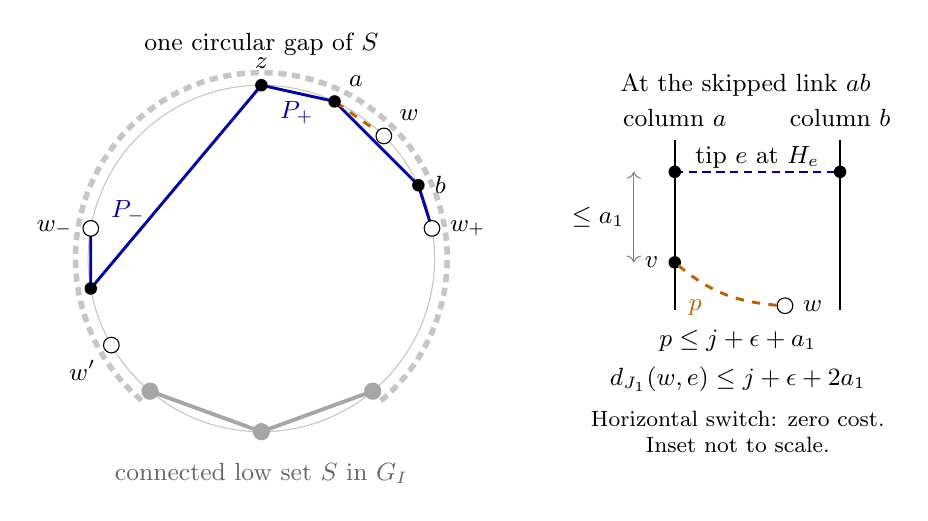
\begin{tikzpicture}[x=1cm,y=1cm,font=\small,
  vertex/.style={circle,fill=black,inner sep=1.6pt},
  seed/.style={circle,draw=black,fill=white,inner sep=2pt},
  low/.style={circle,fill=gray!70,inner sep=2.2pt}]
  \draw[gray!45] (0,0) circle (2.2);
  \draw[gray!45,densely dashed,line width=2pt] (310:2.36) arc (310:590:2.36);
  \node[align=center,fill=white,inner sep=2pt] at (0,2.72) {one circular gap of $S$};
  \coordinate (z) at (90:2.2);
  \coordinate (wm) at (170:2.2);
  \coordinate (q) at (190:2.2);
  \coordinate (wp) at (10:2.2);
  \coordinate (a) at (65:2.2);
  \coordinate (b) at (25:2.2);
  \coordinate (w) at (45:2.2);
  \coordinate (partner) at (210:2.2);
  \coordinate (s1) at (230:2.2);
  \coordinate (s2) at (270:2.2);
  \coordinate (s3) at (310:2.2);
  \draw[gray!70,line width=1.4pt] (s1)--(s2)--(s3);
  \draw[blue!65!black,line width=1.05pt] (z)--node[left,pos=.62] {$P_-$} (q)--(wm);
  \draw[blue!65!black,line width=1.05pt] (z)--(a)--(b)--(wp);
  \node[blue!65!black] at (.45,1.85) {$P_+$};
  \draw[orange!75!black,dashed,line width=1.05pt] (w)--(a);
  \node[vertex,label=above:$z$] at (z) {};
  \node[seed,label=left:$w_-$] at (wm) {};
  \node[vertex] at (q) {};
  \node[seed,label=right:$w_+$] at (wp) {};
  \node[vertex,label=above right:$a$] at (a) {};
  \node[vertex,label=right:$b$] at (b) {};
  \node[seed,label=above right:$w$] at (w) {};
  \node[seed,label=below left:$w'$] at (partner) {};
  \foreach \s in {s1,s2,s3} {\node[low] at (\s) {};}
  \node[gray!80!black,below] at (0,-2.48) {connected low set $S$ in $G_I$};

  \begin{scope}[shift={(5.25,.05)}]
    \node[align=center] at (.9,2.15) {At the skipped link $ab$};
    \draw[thick] (0,-.7)--(0,1.45);
    \draw[thick] (2.1,-.7)--(2.1,1.45);
    \node[above] at (0,1.5) {column $a$};
    \node[above] at (2.1,1.5) {column $b$};
    \draw[blue!65!black,densely dashed,line width=.9pt] (0,1.05)--(2.1,1.05);
    \node[above,fill=white,inner sep=1pt] at (1.05,1.05) {tip $e$ at $H_e$};
    \node[vertex] at (0,1.05) {};
    \node[vertex] at (2.1,1.05) {};
    \node[vertex,label=left:$v$] at (0,-.1) {};
    \node[seed,label=right:$w$] (wi) at (1.4,-.65) {};
    \draw[orange!75!black,dashed,line width=1.05pt] (wi) to[bend left=18] node[below left,pos=.6] {$p$} (0,-.1);
    \draw[<->,gray] (-.52,-.1)--node[left,black] {$\le a_1$} (-.52,1.05);
    \node[align=center] at (.8,-1.35) {$p\le j+\epsilon+a_1$\\[3pt]$d_{J_1}(w,e)\le j+\epsilon+2a_1$};
    \node[align=center,font=\footnotesize] at (.8,-2.25) {Horizontal switch: zero cost.\\Inset not to scale.};
  \end{scope}
\end{tikzpicture}
\caption{The key step in Proposition~\ref{pack:bound}, shown for a
surviving seed $w$. In a gap of the connected low set $S$, an extreme
path skips the column of $w$ by the terminal link $ab$. The witness
partner $w'$ is outside the small ball and lies strictly outside the
closed interval $[a,b]$.
The descending path from $w$ must first reach $a$ or $b$; call that point
$v$. Only this first prefix is shown in orange dashes.
Survival of the low-tip test gives $s(e)\ge s(w)-j$, forcing the
short prefix estimated in the inset. Blue paths use $G_{J_2}$; connections
of $S$ may use the larger graph $G_I$. The circular drawing records column
order, not metric lengths; extreme paths need not be monotone in that order.}
\label{fig:surviving-seeds}
\end{figure}


\begin{remark}
\label{pack:purpose}
The bounded number of nearby seed groups has two uses. Independent
group coins can isolate one group's proposal at a pair, and only
boundedly many families of random formulas can compete on a small ball.
The first use gives secondary separation; the second preserves the
common charts needed at later scales. The conclusion applies to seeds
of the surviving witness pairs. It does not assert bounded overlap of
all broad-band cells or their full neighborhoods: padded cells separate
the chosen seeds, and exclusion of the component barriers brings those
seeds close to the two short paths.
\end{remark}

\section{Ordered fields and separation on the two arcs}
\label{ord:section}

The packing bound limits the number of secondary proposals that can
affect any one small ball. We now supply the scalar fields used by those
proposals and by
their final separation test. We use the circular order and the
noncrossing links of the column model.
All fields in this section are defined on a whole band $X_I$, including
its separate components. A bound for vertical Lipschitz constants,
together with compatibility at switches, implies the same bound for
the intrinsic distance $d_I$ wherever that distance is finite.

This section provides two tools.  First, a point-distance function has a
supporting field that is monotone toward a specified target along both
circular arcs and retains the exact distance at that target.  Second,
short paths on which the field rises and falls in a sufficiently thin band
force a distant pair with nearly equal field values onto opposite arcs.  A
signed transverse field will then distinguish the pair.

\subsection{Ordered supports of point distances}

\begin{definition}\label{ord:definition}
Let $a,b$ be two distinct column indices. A real field $s$ on $X_I$ is
\emph{ordered from $a$ to $b$}, with slope bound $M$, if it respects
every switch, is $M$-Lipschitz on every vertical column, and, at each
height $H\in I$, is nondecreasing on each of the two circular arcs
oriented from $a$ to $b$. In particular, the value on column $a$ is a
global minimum at that height, and the value on column $b$ is a global
maximum. We call the two open arcs the positive and negative arcs,
with either assignment of these names.
\end{definition}

Adding a constant to an ordered field preserves its order and slope
bound. Multiplication by a positive constant multiplies the slope
bound by that constant. Its negative is ordered after interchanging
the two boundary columns. A field depending only on height is
ordered for any choice of distinct boundary columns.

The supporting field below is obtained by taking running minima toward
the target column on each arc.  Connected distance sublevels are what make
this operation compatible with the switches.

\begin{lemma}[Ordered support of a point distance]\label{ord:support}
Suppose that $k,w$ belong to one component of $X_I$. There is an
ordered field $L$ of slope bound $1$ such that
\[
 L(k)=0,\qquad L(w)=d_I(k,w),\qquad
 L(v)\le d_I(k,v)\quad(v\in X_I),
\]
where the last inequality uses the convention that distance to a
different component is infinite.
\end{lemma}

\begin{proof}
Put $D=d_I(k,w)$. If $D=0$, the constant zero field suffices. If $k,w$
have representatives on the same column, then
$D=|h(w)-h(k)|$ and the field
\[
 L(v)=\min\{|h(v)-h(k)|,D\}
\]
suffices, with any two distinct indices as boundary columns: vertical travel attains this distance on that column, and
every path has length at least its absolute height change.

Otherwise choose a representative column $a$ of $k$ and a different
representative column $b$ of $w$. Write
\[
 f_i(H)=\min\{d_I(k,(i,H)),D\},\qquad H\in I,
\]
where $f_i=D$ on any component not containing $k$. Every $f_i$ is
$1$-Lipschitz, and the values respect switches. Moreover,
\[
 f_a(H)=\min\{|H-h(k)|,D\}=\min_i f_i(H).
\tag{\ref{ord:support}.1}\label{ord:root-minimum}
\]

For fixed $H$ and $t\le D$, every nonempty strict sublevel
\[
 S_t(H)=\{i:f_i(H)<t\}
\]
is connected in the active column graph and contains $a$. To see
this, let $i\in S_t(H)$ and take a path from $k$ to $(i,H)$ of length
less than $t$. If the path visits column $z$ at height $T$, its
remaining length is at least $|T-H|$. Its prefix followed by vertical
travel on $z$ to height $H$ therefore has length less than $t$.
Thus every visited column belongs to $S_t(H)$, and projection of
these paths to column indices connects $S_t(H)$ to $a$.

Consider a link with distinct endpoints $p,q$ at height $H$, and put
$c=f_p(H)=f_q(H)$. If neither endpoint is $a$, let $[p,q]_a$ be the
closed circular interval from $p$ to $q$ that does not contain $a$.
Then
\[
 f_z(H)\ge c\qquad(z\in[p,q]_a).
\tag{\ref{ord:support}.2}\label{ord:collision}
\]
Indeed, a strict-sublevel path from any column $z$ with $f_z(H)<c$
to $a$ avoids $p,q$, whereas Lemma~\ref{geo:chord-separation}
forbids such a path when $z$ is strictly inside $[p,q]_a$.
If one endpoint is $a$, both endpoint values equal the global
minimum in \eqref{ord:root-minimum}.

Cut the circular order at $a$. For $i\ne a$, let $[i,b]_a$ denote
the closed interval between $i$ and $b$ in the resulting linear
order, and define
\[
 L(i,H)=\min_{z\in[i,b]_a} f_z(H),\qquad
 L(a,H)=f_a(H).
\tag{\ref{ord:support}.3}\label{ord:projection}
\]
These are finite minima of $1$-Lipschitz functions. Along either
arc from $a$ to $b$ the intervals in \eqref{ord:projection} shrink,
so their minima are nondecreasing; the initial root value is a
lower bound for all of them by \eqref{ord:root-minimum}.

We check switches explicitly. If a link meets $a$, its other
endpoint has the global minimum value, and so does its value of
$L$. Otherwise order its endpoints as $p<q$ in the order cut at
$a$. By \eqref{ord:collision} the minimum of $f$ on $[p,q]_a$ is
their common value $c$. If $b$ lies between $p$ and $q$, both
minima defining $L(p,H),L(q,H)$ equal $c$. If $b$ lies outside
that interval, the longer of the two minimizing intervals is the
union of the shorter one and $[p,q]_a$. The minimum on the
shorter interval is at most $c$, because it contains a link
endpoint. The two minima are again equal. Thus $L$ respects
every switch and is an ordered field on the quotient.

Finally, $L(i,H)\le f_i(H)\le d_I(k,(i,H))$. At $k$, its
root value is zero. At $w$, the minimizing interval is the
singleton $\{b\}$ and its value is $D$.
\end{proof}

\subsection{A transverse coordinate}

At a fixed height the ordered field increases from $a$ to $b$ along both
arcs. Equal values can therefore occur on opposite arcs. The next field
records the side and vanishes wherever a switch can change sides.

\begin{definition}\label{ord:transverse-definition}
Let $s$ be ordered from $a$ to $b$ with slope bound $4$. In
$\R^2$ define the set
\[
 \begin{split}
 Z_s={}&\{(s(a,H),H),(s(b,H),H):H\in I\}\\
 &{}\cup\{(s(p,H),H): H\in I\cap S_{pq},\
     p\text{ and }q\text{ lie on opposite open arcs}\}.
 \end{split}
\]
For a representative $(i,H)$ define
\[
 t_s(i,H)=
 \begin{cases}
  \dist_\infty((s(i,H),H),Z_s),&i\text{ on the positive arc},\\
  -\dist_\infty((s(i,H),H),Z_s),&i\text{ on the negative arc},\\
  0,&i\in\{a,b\}.
 \end{cases}
\]
Here $\dist_\infty$ is distance for the maximum norm on $\R^2$.
\end{definition}

\begin{lemma}\label{ord:transverse-lipschitz}
The field $t_s$ is well defined on $X_I$, respects all switches,
and is $4$-Lipschitz for $d_I$.
\end{lemma}

\begin{proof}
The image of $H\mapsto(s(i,H),H)$ has Lipschitz constant at most
$4$ for the maximum norm, and distance to a fixed nonempty set
is $1$-Lipschitz. Thus $t_s$ is vertically $4$-Lipschitz on
each open-arc column; it is identically zero on each boundary
column. At a switch between columns on the same open arc, its
values agree because both $s$ and height agree. At a switch
between opposite open arcs the common coordinate image belongs
to $Z_s$, so both values vanish. At a switch involving a boundary
column, its image belongs to $Z_s$ for the same reason. These
checks also prove independence of representatives. Summing along
any finite path of vertical motions and switches proves the
$d_I$ bound.
\end{proof}

\subsection{Field excursions force opposite arcs}

The next observation records the crossing argument with its height
error. A path here can be a subpath of a concatenation; saying
that it stays within length $A$ of a point means that every point
on it can be joined to that point by a path of length at most $A$
in $X_I$. This condition holds, for example, for any
subpath of the union of two paths of length at most $A$ issuing
from that point.

\begin{lemma}[Overlapping traversals on one arc]\label{ord:overlap}
Let $J\subset I$ have width $\eta$. Suppose that $s$ is ordered
with slope bound $4$, and that paths $\Gamma_x,\Gamma_y$ in
$X_J$ use only columns of the same open arc. Assume that
$\Gamma_x$ stays within length $A_x$ of $x$ and $\Gamma_y$
stays within length $A_y$ of $y$. If the range of $s$ on each
path contains an interval $[u,v]$ with
\[
 v-u>32\eta,
\]
then
\[
 d(x,y)\le A_x+A_y+2\eta.
\]
\end{lemma}

\begin{proof}
Restrict and orient each path so that its endpoint values are
$u$ and $v$. Fix $H_*\in J$ and write $q_i=s(i,H_*)$.
The values $q_i$ are nondecreasing in the linear order on this
open arc, and
\[
 |s(i,H)-q_i|\le4\eta\qquad(H\in J).
\tag{\ref{ord:overlap}.1}\label{ord:profile-error}
\]
Choose a point on $\Gamma_x$ of value $c=(u+v)/2$, with
representative column $i$. Then $|q_i-c|\le4\eta$.
The initial column of $\Gamma_y$ has reference value at most
$u+4\eta<q_i$, and its terminal column has reference value
at least $v-4\eta>q_i$. Its column word therefore starts
strictly before $i$ and ends strictly after $i$.

If $\Gamma_y$ visits column $i$, connect the two visits on
that column vertically at cost at most $\eta$, giving the
claim. Otherwise Lemma~\ref{geo:skipping} supplies a switch
on $\Gamma_y$ with endpoint columns $p<i<q$. If its height
is $H_0\in J$, then
\[
 |q_p-q_q|\le8\eta,
 \qquad q_p\le q_i\le q_q.
\]
In particular both endpoint reference values differ from
$q_i$ by at most $8\eta$. The two endpoints of $\Gamma_x$
have reference values respectively at most $u+4\eta$ and
at least $v-4\eta$. Since $(v-u)/2>16\eta$, these lie
strictly below $q_p$ and strictly above $q_q$, respectively.
Thus the middle point on column $i$ is strictly inside the
interval bounded by the link $pq$, whereas the endpoints
of $\Gamma_x$ are strictly outside it.
Lemma~\ref{geo:chord-separation} implies that $\Gamma_x$
visits $p$ or $q$. Connect this visit vertically to height
$H_0$ and, if needed, use the zero-cost switch $pq$.
This joins a point of $\Gamma_x$ to a point of $\Gamma_y$
at cost at most $2\eta$ (in fact $\eta$ suffices when
using the visited endpoint of that switch). The assumed
connections to $x,y$ complete the proof.
\end{proof}

\begin{lemma}[Quantitative separation on the two arcs]\label{ord:two-side}
Set $R=10^{-8}$. Let $s$ be an ordered field of slope bound
$4$ on $X_I$. Suppose that $x,y\in X_I$ satisfy
\[
 1\le d(x,y)\le2,\qquad d_I(x,y)=d(x,y),
 \qquad |s(x)-s(y)|\le10^{-3}R.
\]
Let $J\subset I$ be a common height interval of width
\[
 \eta\le10^{-6}R
\]
containing $x,y$. For each $z\in\{x,y\}$, suppose that
there are two paths $\gamma_z^-,\gamma_z^+$ in $X_J$,
starting at $z$, of length at most $2R$, whose terminal
points $z^-,z^+$ satisfy
\[
 s(z^-)<s(z)-0.4R,\qquad s(z^+)>s(z)+0.4R.
\]
Then $t_s(x),t_s(y)$ have opposite signs and
\[
 0.01R\le |t_s(x)|,|t_s(y)|\le8.
\]
\end{lemma}

\begin{proof}
Write $s_0=s(x)$ and $H_x=h(x)$. We first prove that $Z_s$
does not meet the rectangle
\[
 \mathcal Q=
 [s_0-0.2R,s_0+0.2R]\times
 [H_x-0.02R,H_x+0.02R].
\tag{\ref{ord:two-side}.1}\label{ord:empty-rectangle}
\]
Suppose otherwise that $(c,H_0)\in Z_s\cap\mathcal Q$.
At the reference height $H_0$, the endpoint columns of
each low path have field value strictly below $c$, and
the endpoint columns of each high path have value strictly
above $c$. Indeed their terminal values are respectively
below $s_0-0.399R$ and above $s_0+0.399R$, and moving
their values to height $H_0$ changes them by at most
\[
 4(0.02R+\eta)\le0.080004R.
\]
These inequalities leave a strict margin from the interval
$[s_0-0.2R,s_0+0.2R]$.

If $(c,H_0)$ is the image of a boundary column, these
strict inequalities contradict that column's extremality.
Otherwise it is the image of a crosslink with one endpoint
on each open arc. At height $H_0$, monotonicity puts every
column of value less than $c$ on the root side of this
crosslink and every column of value greater than $c$ on
its opposite side. The projected concatenation
$(\gamma_z^-)^{-1}\gamma_z^+$ must therefore visit an
endpoint of the crosslink by
Lemma~\ref{geo:chord-separation}. Each such visit is
reachable from $z$ in length at most $2R$, since it lies
on one of the two original paths. Move vertically from
the two visits to height $H_0$ and use the crosslink if
needed. This produces an $x$--$y$ path of length at most
\[
 4R+2(0.02R+\eta)<1,
\]
contradicting $d(x,y)\ge1$. This proves
\eqref{ord:empty-rectangle}.

The maximum-norm ball of radius $0.01R$ around either
$(s(x),h(x))$ or $(s(y),h(y))$ is contained in
$\mathcal Q$. Hence
\[
 |t_s(x)|,|t_s(y)|\ge0.01R.
\tag{\ref{ord:two-side}.2}\label{ord:positive-magnitude}
\]
In particular both centers have representatives on open
arcs, with a well-defined choice of arc.

Consider the value strip
\[
 \mathcal S=\{v\in X_J: s_0-0.18R\le s(v)
                                      \le s_0+0.18R\}.
\]
No representative of a point of $\mathcal S$ is on a
boundary column, and no switch in $\mathcal S$ joins
opposite open arcs. Either event would give an image in
$Z_s\cap\mathcal Q$, because its height belongs to $J$
and its value is within $0.18R$ of $s_0$. Thus any path
contained in $\mathcal S$ remains on a single open arc.

For $z=x,y$, the concatenation
$(\gamma_z^-)^{-1}\gamma_z^+$ starts below the strip
and ends above it. The scalar field is continuous along
this path, including at switches. Take its first visit
to the upper strip boundary, and its last visit to the
lower strip boundary preceding that visit. The intervening
subpath $\Gamma_z$ stays in $\mathcal S$, traverses its
full value interval, and lies on one open arc. Every
point on it is reachable from $z$ in length at most $2R$.
If $\Gamma_x,\Gamma_y$ were on the same arc,
Lemma~\ref{ord:overlap}, with common interval of length
$0.36R>32\eta$, would give
\[
 d(x,y)\le4R+2\eta<1.
\]
Consequently their two arcs are opposite.

It remains to relate these full traversals to the centers.
From either center $z$, follow either one of its two
original paths until its first exit from $\mathcal S$.
The resulting initial subpath $\Pi_z$ lies on the
center's arc and its value range contains the interval
between $s(z)$ and the strip boundary it first reaches.
This interval has length at least $0.179R$. All its
points are reachable from $z$ in length at most $2R$.
If the two centers had the same arc, exactly one of the opposite
full traversals $\Gamma_x,\Gamma_y$ would lie on that
arc. If it were $\Gamma_x$, compare it with $\Pi_y$; if
it were $\Gamma_y$, compare it with $\Pi_x$. In either case
the paths come from different centers and their value ranges overlap in
an interval
of length at least $0.179R>32\eta$. Another application
of Lemma~\ref{ord:overlap} gives the same contradiction.
Thus the centers have opposite arcs and, by
\eqref{ord:positive-magnitude}, $t_s(x),t_s(y)$ have
opposite signs.

Finally Lemma~\ref{ord:transverse-lipschitz} and the
assumed equality of band and unrestricted distances give
\[
 |t_s(x)|+|t_s(y)|
   =|t_s(x)-t_s(y)|
   \le4d_I(x,y)=4d(x,y)\le8.
\]
This proves both upper bounds.
\end{proof}


\subsection{Ordered charts in system \texorpdfstring{$B$}{B}}
\label{ord:charts}

Besides ordinary charts, system $B$ uses \emph{ordered charts}. Such a
chart has field
\[
 P=s+\lambda u,
\]
where $s$ is ordered with vertical Lipschitz constant at most $4$ and
$u$ has Lipschitz constant at most $K$ for $d_I$. At the creation of the
chart, $u=0$. The update in Section~\ref{sec:increment} changes $u$ while
preserving this bound. Our choice of $\lambda$ gives
$\Lip(P)\le4+\lambda K<5$ for finite $d_I$, as required by the chart
invariant of Section~\ref{sets:section}.

The band $I$, the ordered part $s$, its two boundary columns and choice
of positive arc, and the label functions $Z,\sigma$ remain fixed in original units for the
lifetime of an ordered identifier. In particular its transverse field
$t_s$ remains fixed. Its region can shrink as other charts replace parts
of it, and its auxiliary field $u$ changes through the prescribed
increments. Thus the current full field $P$ may change without changing
the identifier or the ordered data it records.

\section{The secondary update}
\label{sec:secondary}

We now separate the pairs left by the two tests in
Section~\ref{main:section}. Their endpoints are seeds, grouped by their
broad and narrow bands, their padded $g$-cell, and their two old chart
identifiers. Proposition~\ref{pack:bound} bounds by $M_{\mathrm{pack}}$
the number of these groups meeting a narrow-band ball of radius $4R$.
This lets us isolate one group's clipping at an endpoint with positive
probability. In Section~\ref{pad:assembly}, the same bound will control
the number of formulas competing on a small ball.

Clipping raises the field using a proposal based on distance to admitted
seeds. In an ordinary chart it may also create an ordered chart, whose
auxiliary field starts at zero. For a surviving pair in an ordered chart,
either an endpoint is admitted in some orientation, allowing clipping,
or each endpoint has short paths on which the fixed ordered part rises
and falls. In the latter case Lemma~\ref{ord:two-side} places the
endpoints on opposite arcs, and the increment mode separates them using
the transverse field. Clipping and increment are alternatives at the
current scale; a newly created ordered chart is available for increments
at subsequent scales.

\subsection{Clipping near admitted seeds}
Fix the orientation of the old $B$ chart. In an ordinary chart its
comparison field is $p_*=s$; in an ordered chart it is one of $P$ and $-P$,
chosen fairly and shared by the entire old identifier. For each group
choose a representative $w_c$ and set $p_c=p_*(w_c)$. The weak diameter
bound of its $g$-cell, together with old-chart eligibility, gives
\begin{equation}\label{sec:variation}
 |p_*(w)-p_c|\le60g
 \quad\text{at every seed }w\text{ of the group}.
\end{equation}
All short paths used for this comparison lie in the old field band.

In an ordinary chart choose an ordered support $L$ with
\begin{equation}\label{sec:support}
 L\le p_*,\qquad L(w_c)=p_c,\qquad \Lip_{\mathrm{vert}}(L)\le1,
\end{equation}
using Lemma~\ref{ord:support} with the source of $s$ and target $w_c$.
For a constant chart use $L=0$. All seeds in an ordinary chart are
\emph{admitted}. In an ordered chart admit $w$ in the chosen orientation
if
\begin{equation}\label{sec:admission}
 p_*(v)\ge p_c-0.65R
 \quad\text{whenever }d_{J_2}(w,v)=R.
\end{equation}
The test is vacuous when that sphere is empty. Admission supplies the
boundary comparison needed by the shallow proposal below. Failure in
both orientations will instead supply paths on which the comparison
field rises and falls.
These decisions use no fresh clipping noises.

A group's seeds have $d_{J_1}$-diameter at most $10g$, but may lie in
several components of the narrow band. Give the group one independent
fair coin, and keep its representative $w_c$, value $p_c$, orientation,
and support $L$ (when present) common to all those components. For a kept
group, let $F$ be its admitted seeds in one narrow-band component,
provided this set is nonempty, and put
\[
 d_F(v)=\min_{w\in F}d_{J_2}(w,v).
\]
Apply Theorem~\ref{int:interpolation} to $0.9d_F$ on the entire
component, with error $E_B$, obtaining $Q_F$. Use the resulting proposal
only on $U_F=\{d_F\le R\}$. Thus broad-band smallness controls the
variation within a group, while narrow-band distance controls where
its proposals can act. The shallow branch supplies the gain at seeds.
In an ordinary chart the ordered-support branch protects a boundary where
the old field decreases too fast. The height shield protects the band ends.
Propose on this domain the minimum of
\begin{align}
 T_F(v)&=p_c+0.05R-Q_F(v),\label{sec:shallow}\\
 O_F(v)&=p_c+0.05R+4(L(v)-p_c)+\alpha_F,
             \quad\text{in an ordinary chart only},\label{sec:ordered-branch}\\
 H_F(v)&=\psi_F(h(v)).\label{sec:height-branch}
\end{align}
Here $\alpha_F$ is uniform in $[0,E_B]$ and independent of the fresh
interpolation noises defining $Q_F$. The height shield $\psi_F$
is $p_c-1+\alpha_h$ at the two ends of $J_2$, rises linearly to
$p_c+2+\alpha_h$ within distance $0.09a_2$ of each end, and is constant
on the intervening plateau; $\alpha_h$ is independently uniform in
$[0,E_B]$. Extend it constantly beyond the band. Conditional on the old
charts, bands, groups, orientations, admissions, and group coins, these
interpolation and branch noises are fresh, and the noise families of
different groups are independent. Replace $p_*$ by its maximum with
the proposals of all kept groups on their domains, and convert back to
the old field orientation.

\begin{lemma}[Validity of secondary clipping]\label{sec:validity}
The secondary update preserves the nested-set and chart invariants.
Its movement at each point, measured in symmetric difference, is bounded
by a universal constant in scale units.
\end{lemma}
\begin{proof}
First consider a point with $d_F(v)=R$. The shallow branch satisfies
\[
 T_F(v)\le p_c+0.05R-0.9R+E_B=p_c-0.849R.
\]
In an ordered chart a nearest admitted seed gives
$p_*(v)\ge p_c-0.65R$, leaving a margin of $0.199R$.
In an ordinary chart the same margin applies whenever that last
inequality holds. Otherwise $L\le p_*$ gives
\[
 O_F(v)-p_*(v)
 \le0.05R+3(p_*(v)-p_c)+E_B<-1.899R.
\]
Thus the proposal has a uniform margin below the old field on every
distance boundary. At the height ends the shield gives a margin as well:
each domain point lies within $R$ of a seed, which lies within $10g$ in
$d$ of $w_c$, and the old comparison has Lipschitz constant less than $5$
along these eligible paths. Its difference from $p_c$ is less than
$5(R+10g)<1/2$.

Every domain lies in its old chart, by seed eligibility. The comparison
orientation and label variables are common on overlapping domains.
Extend each proposal, after clamping against the old field, by the old
field off its domain. The boundary margins and the clipping argument in
Section~\ref{sets:section} show that this extension glues vertically and
respects switches. The finite maximum of these extensions has the same
properties. The spatial branches have Lipschitz constant at most $4$;
the shield has constant $3/(0.09a_2)$, which is less than $1/\kappa_B$.

A winning atom of $Q_F$ gives a constant plus or minus one point-source
distance and hence a fresh ordinary chart on its narrow-band component.
A winning $O_F$ branch, after conversion back to the old orientation,
becomes the ordered part of a new chart on the old band, with $u=0$.
It has slope at most $4$. Additive constants preserve its order; if
conversion negates the comparison field, reverse the two boundary
columns as in Definition~\ref{ord:definition}. This ordered part, its
band, and its arc assignment remain fixed under the new identifier;
subsequent increments change only its auxiliary field.
A height branch is rebased by
Lemma~\ref{sets:vertical}. Unchanged points retain their chart, and uses
of the same inherited atom in the same interpolation keep one identifier.

Finally $Q_F$ lies within $E_B$ of $0.9d_F$. Thus the shallow branch is
at most $p_c+0.051R$ and the old field is within $5(R+10g)$ of $p_c$
where the group can act. Taking a maximum over any number of groups does
not add these bounds. Formula~\eqref{sets:distance} gives a uniform
symmetric-difference movement bound.
\end{proof}

\begin{lemma}[Separation at admitted seeds]\label{sec:admitted-success}
If a surviving pair has a seed admitted for one comparison orientation,
then the no-change and secondary-clipping modes together give a probability
bounded below by a positive universal constant of separating that pair by
a positive universal amount.
\end{lemma}
\begin{proof}
At an admitted seed $w$, $|Q_F(w)|\le E_B$. Equations
\eqref{sec:variation}--\eqref{sec:support} imply that every applicable
spatial branch exceeds $p_*(w)+0.04R$: for the ordered branch use
$|L(w)-p_c|\le10g$. The height shield is on its interior plateau.
The other pair endpoint is outside this group's update domains, because
the group's seeds have unrestricted diameter at most $10g$ and the pair
distance is at least one.

At either endpoint all groups that could act have a seed within $R$ in
the narrow band. At most $2M_{\mathrm{pack}}$ groups can therefore act in total at the two endpoints.
Keeping the designated group and suppressing all other such groups has
probability at least $2^{-(2M_{\mathrm{pack}}+1)}$, a convenient lower bound. The desired ordered orientation,
when needed, has probability $1/2$.

Let $B_x,B_y$ denote the old system-$B$ sets and $B'_x,B'_y$ the updated sets.
On this event one endpoint is unchanged, while the movement of the other
has measure at least $0.04\kappa_BR$. If
$\mu(B_x\mathbin\triangle B_y)\ge0.01\kappa_BR$, the no-change mode
already gives the required separation. Otherwise the triangle inequality
gives $\mu(B'_x\mathbin\triangle B'_y)>0.03\kappa_BR$, and in
particular at least $0.02\kappa_BR$.
Each mode has probability $1/4$, so both alternatives have uniform
positive probability.
\end{proof}

\subsection{The increment in ordered charts}\label{sec:increment}
For an ordered identifier, the ordered part $s$, its band $I$, and its
arc assignment stay fixed while the auxiliary field $u$ changes and the
current region $\mathcal R$ may shrink. Its transverse field $t_s$ is
therefore fixed as well. We define the increments in original length
units, so these stored fields do not change when a step is analyzed in
units of its scale.

Define a continuous trapezoidal function $H:[0,\infty)\to[0,1]$ which vanishes
off $[0.005R,10]$, equals one on $[0.01R,8]$, and is linear on the two
remaining intervals. At scale $r$, in original units, add to $u$ the
function
\begin{equation}\label{sec:increment-formula}
 \pm t_s(v) H(|t_s(v)|/r)
 \min\{1,d(v,X\setminus\mathcal R)/r\}.
\end{equation}
The sign is fair and common to the old identifier. When the complement is
empty its distance factor is one. The formula is defined on the chart's
whole band, with changes to the sets effective only in its current region.
Old terms of $u$ are retained without modification.

\begin{lemma}[Increment bound]\label{sec:increment-bound}
If $Q>2000/R$, all increments of one ordered identifier together have
$d_I$-Lipschitz constant at most $K=100$. They preserve the nested sets,
introduce no chart interfaces, and move each point by at most a universal
constant times the scale.
\end{lemma}
\begin{proof}
The function $t_s$ is $4$-Lipschitz in $d_I$. The scalar function
$t\mapsto tH(|t|/r)$ has Lipschitz constant at most $6$ and magnitude
at most $10r$. The distance factor has Lipschitz constant at most $1/r$
for $d$, hence for $d_I$. Each increment has Lipschitz constant at most
$24+10=34$.

Its support is contained in
$0.005Rr<|t_s|<10r$. Since $t_s$ is fixed for this identifier, the
support intervals at distinct scheduled scales are disjoint when
$Q>2000/R$. In a comparison of two points at most two summands are
nonzero at either endpoint. Subtracting their zero values at the other
endpoint if necessary bounds the difference by $68d_I(v,w)$. Thus
$\Lip(u)\le68<K$ at all times.

The distance factor makes the movement vanish continuously at the region
boundary. Inside the region the new field has Lipschitz constant at most
$4+\lambda K<5<1/\kappa_B$. The vertical gluing argument applies, and
the region partition does not change. The amplitude bound is $10r$ before
the factor $\lambda$, proving the last assertion.
\end{proof}

\begin{lemma}[The remaining pairs]\label{sec:remaining}
Suppose a surviving pair has no admitted endpoint in either ordered
orientation. Then the increment mode separates it by a positive universal
amount with uniformly positive probability.
\end{lemma}
\begin{proof}
Normalize the current scale to one. Ordinary charts admit every seed,
so the old $B$ chart is ordered. Failure of each admission test supplies
a point on the corresponding $d_{J_2}$-sphere of radius $R$ and an
attaining path of length $R$. Failure for $P$ supplies a decrease of
$P$, and failure for $-P$ supplies an increase. By
\eqref{sec:variation}, each change has magnitude greater than
$0.65R-60g$. The correction $\lambda u$ changes by at most
$\lambda KR$ on either path. Thus the ordered part $s$ has a positive
and a negative change of magnitude greater than
\[
 0.65R-60g-\lambda KR>0.4R
\]
along these paths from each endpoint.

A shortest $x$--$y$ path has length at most $2$ and stays in the eligible
radius-$5$ ball, hence in the old band $I$. This proves
$d_I(x,y)=d(x,y)$ and bounds the change of $u$ by $2K$. The $B$ cutoff
therefore gives
\[
 |s(x)-s(y)|\le10^{-4}R+2\lambda K<0.001R.
\]
The four excursion paths lie in the common band $J_2$, whose width
satisfies Lemma~\ref{ord:two-side}. Applying that lemma gives opposite
signs of $t_s$ and $0.01R\le |t_s(x)|,|t_s(y)|\le8$.

These bounds put both endpoints on the plateau of the trapezoidal
factor. Eligibility also puts their radius-$5$ balls in the current
region, so the distance factor in \eqref{sec:increment-formula} equals
one at both endpoints. For one of the two increment signs,
\[
 |P_{\mathrm{new}}(x)-P_{\mathrm{new}}(y)|
   \ge \lambda|t_s(x)-t_s(y)|\ge0.02\lambda R.
\]
Formula~\eqref{sets:distance} proves separation at least
$0.02\kappa_B\lambda R$. The favorable sign has probability at least
$1/2$.
\end{proof}

\section{Preserving charts and assembling the embedding}
\label{pad:assembly}

The local constructions now provide a uniform chance of separation at a
pair's distance scale. Two estimates let us use that chance in a complete
schedule: coarser scales rarely destroy the common charts required by the
test, and finer scales move too little label mass to erase its certificate.
We first collect these estimates, then choose the scale spacing and write
the resulting finite cut embedding.

\subsection{The one-step estimates}
All constants in this section depend only on the fixed choices in
Section~\ref{sets:parameters}. In particular they are independent of the
number of columns, band components, chart identifiers, and scales.

\begin{proposition}[Movement and success]\label{pad:success}
There are constants $M<\infty$ and $b,p>0$ such that the following hold
at every step of scale $r$.
\begin{enumerate}[label=(\roman*)]
\item At every point of $X$, in either system, the symmetric-difference
movement of the unrefined set is at most $Mr$.
\item Given any past for which a vertex pair at distance in $[r,2r)$ is
eligible, the step has probability at least $p$ of producing one of these
certificates:
\begin{enumerate}[label=(\alph*)]
\item unrefined symmetric-difference separation at least $br$ in one
system;
\item a non-neighbor tip $e$ and a set of labels of measure at least $br$
in system $A$ on which both pair vertices are active and $e$ is inactive,
with the vertices strictly on opposite sides of that link.
\end{enumerate}
\end{enumerate}
\end{proposition}
\begin{proof}
Lemma~\ref{main:validity} bounds movement in the main clipping.
Secondary movement is bounded by Lemma~\ref{sec:validity}; increments are bounded by
Lemma~\ref{sec:increment-bound}. These estimates apply even at points
outside the finite vertex list. There are no simultaneous main updates
at a point except at cell overlaps, where every update is unchanged.
Secondary updates take a maximum, whose movement is bounded without
summing over groups. Taking the largest of the bounds gives $M$.

Work in scale units. If one of the cutoffs in
\eqref{sets:cutoffs} fails, no change preserves separation at least the
minimum of $10^{-4}a_2,\kappa_AE_A,\kappa_B10^{-4}R$.
Otherwise the interior requirements hold with probability at least $1/4$.
Conditional on the bands and cells, a missing descending path is handled
by Corollary~\ref{main:pair-separation}: keep that endpoint's cell and suppress the other,
giving positive separation with probability at least $1/4$ conditional
on the main mode. If both paths exist, an excluded pair has the component
certificate on a label set of measure at least $\kappa_Aj/4$, which the
no-change mode preserves.

For a surviving pair, admission at an endpoint is handled by
Lemma~\ref{sec:admitted-success}, including its no-change alternative.
If neither orientation admits either endpoint, apply
Lemma~\ref{sec:remaining}. Each case uses one of four modes, at most one
fair orientation, and at most $2M_{\mathrm{pack}}+1$ prescribed group coins. It follows,
for example, that $p=2^{-(2M_{\mathrm{pack}}+10)}$ is a permissible lower bound after
all interior and mode probabilities. Choose $b>0$ below all the finitely
many displayed gains and certificate masses. These choices depend only
on the fixed parameters.
\end{proof}

\subsection{The probability of splitting a small ball}
The following estimate concerns chart identifiers, not cut components.
System $A$ is refined only after all the updates.

\begin{proposition}[Chart persistence]\label{pad:persistence}
There exist constants $C_0<\infty$ and $\rho_0>0$ such that the following
holds. Condition on the past at a step of scale $r$. Suppose a fixed
closed ball $B_d(v,\rho r)$ lies in a single old region in each system.
For $0<\rho\le\rho_0$, the probability that this ball is split between
different new regions in either system is at most
\begin{equation}\label{pad:loss}
 C_0(\rho+\eta_0).
\end{equation}
Here $\eta_0$ is the relative mesh allowance from
Section~\ref{sets:setup}.
\end{proposition}
\begin{proof}
Normalize $r=1$ and write $B=B_d(v,\rho)$. Every point of $B$ has
a shortest path to $v$ contained in $B$. Joining two such paths gives
a path of length at most $2\rho$ between any two points of $B$.
We will use these paths for all band-distance comparisons.

There are two ways an update could give different chart identifiers on
$B$: its domain could end inside the ball, or different formulas could
win there. Strict margins at domain boundaries prevent the first kind
of change. The comparison estimate of Corollary~\ref{int:comparisons}
controls the second.

\paragraph{Height bands.}
The probability that an endpoint of either random height tiling lies
within $\rho$ of $h(v)$ is $O(\rho+\eta_0)$. Exclude this event and
condition on the tilings. The ball lies wholly in one component of a
broad band and one component of a narrow band: all its center paths
are paths in those bands.
For clipping, each such band is either processed in its entirety or left unchanged.
A narrow band not contained in a broad band has no secondary seeds,
so secondary clipping also leaves it unchanged.

\paragraph{Main clipping.}
Condition further on the radial cells and their coins. Suppose first
that $B$ meets more than one width-$D$ cell, including through different
representatives of a quotient point. For any touched cell $C$ and any
$w\in B\cap C$, a path through the center to a point in another cell
reaches a frontier point $z\in B\cap\partial C$ within length $2\rho$.
If $C$ is available, its old comparison field is the common old field
on $B$. Thus
\[
 F_C(w)\le s(z)+(1-\zeta_A)d_{J_1}(w,z)-3E_A
          \le s(w)+4\rho-3E_A.
\]
For $\rho_0<E_A/10$ the proposal cannot raise the field anywhere on
$B\cap C$. Unavailable cells are unchanged as well. Hence the whole
ball retains its old identifier. In particular we do not need to
exclude a random radial boundary crossing.

It remains to consider a ball lying in one cell $C$. If that cell is
unavailable or its coin is suppressed, it is unchanged. Otherwise its
comparison expression on $B$ is
\[
 \max\{s,\min\{F_C,p_{h,C}\}\}.
\]
Here $F_C=\widetilde p_C-4E_A$ is one interpolation construction,
$p_{h,C}$ is a fixed height function plus its independent offset, and
$s$ is the only branch with no fresh noise. The input $p_C$, portals,
and bands have all been fixed before these noises are sampled.
Every center path has length at most $\rho$ in the interpolation band
and in the old chart band. Corollary~\ref{int:comparisons}, with the
fixed Lipschitz bound of the height function, therefore gives one
winning branch and, if that branch is the interpolation, one named atom throughout $B$,
except with conditional probability $O(\rho+\eta_0)$.
A common old branch retains its identifier; a common spatial atom or
height branch gives a common new chart. At interpolation layer seams
the inherited atom keeps its name, as required by the interpolation
theorem.

\paragraph{Secondary clipping.}
Condition on the cells, surviving groups, comparison orientations,
admissions, and group coins. These choices precede the fresh clipping
noises. A group whose domain meets $B$ has an admitted seed at band
distance at most $R+2\rho<4R$ from $v$. Proposition~\ref{pack:bound}
therefore bounds the number of such groups by $M_{\mathrm{pack}}$.

If a group's domain meets but does not contain $B$, its boundary is
reached within length $2\rho$ from every point of its domain in the
ball. Lemma~\ref{sec:validity} puts the proposal below the old field
at this spatial boundary by a fixed positive margin; height-boundary
crossings have already been excluded. The fixed Lipschitz constants
of the proposal branches and the old field extend this nonaction to
the domain's intersection with the ball when $\rho_0$ is small enough.
Outside the domain there is no update by definition. Discard such a group. Every
remaining relevant domain contains $B$, so its proposal is described
by one fixed expression throughout the ball.

Each relevant domain lies in its seed's old chart and meets $B$.
Since regions partition $X$, that chart must be the ball's common old
chart. Thus all these proposals use the same old comparison orientation
and label variables. The ball lies in one narrow-band component, so
each group contributes only the interpolation for that component. Their
combined expression is the maximum of $p_*$ and the group proposals,
each proposal being the minimum of $T_F$, $H_F$, and, in an ordinary
chart, $O_F$. The $T_F$ are signed, shifted interpolation functions;
the $H_F$ and $O_F$ have independent additive offsets. The only input
without fresh noise is the old field $p_*$. The group data and the
interpolation inputs are already fixed, and fresh noise families are
independent between groups. All center paths are permitted in their
narrow-band metrics and in the old chart band.

Apply Corollary~\ref{int:comparisons} to this expression. Each
interpolation contributes its bounded list of candidate atom names;
the number of lists is bounded by $M_{\mathrm{pack}}$. All constants
are therefore uniform in the graph and the past. Except with
conditional probability $O(\rho+\eta_0)$, one branch and, where
applicable, one atom name wins throughout $B$. The resulting chart
identifier is common to the ball. Repeated appearances of an inherited
atom use its interpolation and original atom name, so crossing a
portal collar does not create another identifier.

No-change and increment modes introduce no chart identifiers. Taking
$\rho_0$ smaller than the finitely many bounds used above and summing
the exceptional probabilities proves~\eqref{pad:loss}.
\end{proof}

\subsection{Choice of spacing and the final map}
Choose $Q=2^m$ large enough for the support condition in
Lemma~\ref{sec:increment-bound}, for $20/Q<\rho_0$, and for
\begin{equation}\label{pad:spacing}
 \frac{40C_0}{Q-1}<\frac12,
 \qquad \frac{6M}{Q-1}<\frac b2.
\end{equation}
Choose the mesh allowance so that $\eta_0\le r_f/r$ for every
pair of scales $r_f<r$ in the finite collection of schedules. Then the
mesh term in \eqref{pad:loss} is no larger than the corresponding scale
ratio. This choice does not change any of the constants above.

Fix a pair and its designated scale $r_f$, and consider
$B_d(x,20r_f)$. Initially it has one chart in each system. Conditional
on having retained that property up to a coarser scale $r$, its first
loss probability is at most $40C_0 r_f/r$. Therefore
\[
 \Pr[\text{a first loss before }r_f]
 \le40C_0\sum_{k\ge1}Q^{-k}<\frac12.
\]
On the complementary event the pair is eligible at scale $r_f$.
Furthermore any $D$-cell needed for its main update has its entire
$1$-neighborhood inside this ball: its weak diameter is at most $10D$.
The old chart bands contain the short paths used in all tests.

By Proposition~\ref{pad:success}, conditional on this event the scale
produces a certificate with probability at least $p$. Subsequent
unrefined movement at any one point is deterministically at most
\[
 M\sum_{k\ge1}r_fQ^{-k}=\frac{Mr_f}{Q-1}.
\]
An ordinary pair separation loses at most twice this quantity. For a
component certificate, remove labels whose membership later changes
at either vertex or at its tip; their total measure is at most three
times this quantity. At least $br_f/2$ of the original certificate
therefore remains. Lemma~\ref{sets:component-refinement} gives final
separation for all those labels, regardless of changes elsewhere.
In either case the final sum of the refined $A$ distance and the
unrefined $B$ distance is at least $br_f/2$ on the successful event.
Its expectation in the designated schedule is consequently at least
\[
 \frac12\,p\,\frac{br_f}{2}
 \ge\frac{pb}{8}d(x,y).
\]

The designated schedule is the residue class containing the dyadic
exponent of $r_f$; every other schedule contributes a nonnegative
distance. Mix uniformly over the $m$ schedules. Within each schedule use the
probability law of the random construction, weighting each outcome by
its probability. More precisely, an outcome is a branch of the finite
execution tree, and its weight is the product of the conditional
probabilities of the choices along that branch. These weights sum to one
even though later geometric choices depend on earlier outcomes.
Take the finite direct sum of their measure spaces
with these weights, and of the two systems. Subtract the
assignment at a fixed reference vertex in every summand. By
Lemma~\ref{sets:component-refinement} the resulting map $F$ is into a
real $L_1$ space and satisfies
\[
 \frac{pb}{8m}d(x,y)\le\|F(x)-F(y)\|_1\le2d(x,y)
 \qquad(x,y\in V).
\]
This map can be written using finitely many cut coordinates. For every
final outcome and every label in system $B$, record the subset of $V$
that is active. For system $A$, record separately, for each active column
component, the subset of original vertices active in that component.
Each such subset $S$ contributes the cut distance
$|\1_S(x)-\1_S(y)|$. Integrating over the labels and averaging with the
schedule and outcome weights therefore gives numbers $w_S\ge0$ such that
\[
 \|F(x)-F(y)\|_1
   =\sum_{\varnothing\ne S\subsetneq V}
       w_S|\1_S(x)-\1_S(y)|.
\]
Empty and full subsets contribute zero and have been discarded. Every
remaining weight is finite: if $x\in S$ and $y\notin S$, its contribution
is bounded by the already established upper bound $2d(x,y)$. Hence
\[
 v\longmapsto\bigl(w_S\1_S(v)\bigr)_{
                         \varnothing\ne S\subsetneq V}
\]
is a map into a finite-dimensional real $\ell_1$ space with exactly the
same distances as $F$.

The column realization identifies these distances with the original
$d_G$. Rescale $F$ by $8m/(pb)$ to obtain Theorem~\ref{thm:main} with
$C=16m/(pb)$. If $V$ has a single point use the zero map. Every constant
is independent of the graph size and of its positive edge lengths.

\section{A consequence for almost-embeddable families}
\label{sec:consequences}

Lee and Sidiropoulos reduce their fixed-parameter almost-embeddable
families to planar and bounded-treewidth pieces joined at single
vertices~\cite[Theorem~1.7]{LS09}. We combine this reduction with
Theorem~\ref{thm:main} and the bounded-treewidth embedding theorem
of the companion~\cite[Theorem~1.1]{Treewidth108}.

A $1$-sum joins two graphs by identifying one vertex of each.
A stochastic embedding of distortion $D$ is a distribution of maps
into graph metrics that do not contract distances, with expected
expansion at most $D$ for every pair.

Informally, the construction of these families starts with a graph drawn
on a compact surface of genus $g$, orientable or nonorientable. One adds
$k$ attachments of prescribed width $w$, called fringes, to $k$ faces,
and then $a$ additional vertices with arbitrary adjacencies; these last
vertices are the apices. In particular, when $k=0$ this includes
bounded-genus graphs with a bounded number of arbitrarily attached
vertices. The corollary uses Lee and Sidiropoulos's named family and
their prescribed attachment and width conventions.

\begin{corollary}[Fixed almost-embeddable families]\label{cor:almost-embeddable}
Fix nonnegative integers $g,k,w,a$, and interpret
$\mathrm{AE}(g,(k,w),a)$ exactly as the almost-embeddable family of
Lee and Sidiropoulos~\cite[Theorem~1.7]{LS09}. Let
$h_0=h_0(g,k,w,a)\in\N_0$ be the target treewidth bound and let
$D=D(g,k,w,a)\ge1$ be a finite stochastic distortion bound supplied there.
Put
\[
 \widehat h=\max\{h_0,1\},\qquad
 K(g,k,w,a)=D\max\{C_{\mathrm{pl}},C_{\widehat h+1}\},
\]
where $C_{\mathrm{pl}}$ is the constant of Theorem~\ref{thm:main}, and
$C_t$ is the companion's constant for bags of cardinality at most
$t\ge2$. Every finite connected simple graph $G$ in this named family,
with strictly positive real edge lengths, admits a map $f$ into a real
$L_1$ space satisfying
\[
 d_G(u,v)\le\|f(u)-f(v)\|_1
 \le K(g,k,w,a)d_G(u,v)\qquad(u,v\in V(G)).
\]
For the same underlying graph, $K(g,k,w,a)$ also bounds the undirected
fractional concurrent flow--cut gap $\phi_*/\lambda_*$ for the finite
nonnegative capacities and demands defined in Section~\ref{intro:flow},
whenever $\lambda_*>0$.
\end{corollary}

\begin{proof}
The singleton case is immediate. Otherwise, replace each input edge length
by the distance between its endpoints; this preserves the metric and gives
reduced positive lengths. Lee--Sidiropoulos Theorem~1.7 stochastically embeds
this metric with distortion at most $D$ into finite $1$-sums of planar graphs
and graphs of treewidth at most $h_0$. Since the companion indexes $C_t$ by
bag cardinality, enlarging $h_0$ to $\widehat h$ gives the applicable constant
$C_{\widehat h+1}$. Put $M=\max\{C_{\mathrm{pl}},C_{\widehat h+1}\}$.

For a connected target piece with nonnegative edge lengths, add $\varepsilon>0$
to every edge and apply Theorem~\ref{thm:main} or the companion theorem.
As $\varepsilon\downarrow0$, the shortest-path matrices converge, so the
corresponding $L_1$ distance matrices have a subsequential limit in the closed
finite cut cone, retaining exactly the bound $M$ and identifying zero-distance
pairs. The finite expected expansion
ensures that all images of the finite input lie in a single finite-distance
target component almost surely. Lemma~1.5 of~\cite{LS09} retains the bound
$M$ on finite $1$-sums, and its Lemma~1.2 composes this bound with the
stochastic distortion $D$, giving $K=DM$. Applying the same cut-cone limit
to input lengths, followed by the fixed-graph equality
of~\cite[Section~3, Theorem~3.2]{GNRS04}, gives the flow--cut conclusion.
\end{proof}

This corollary concerns only the cited fixed-parameter almost-embeddable
families. It does not establish closure under general clique sums of order
greater than one, and therefore does not prove the full GNRS conjecture.

\bibliographystyle{plain}
\bibliography{references}
\end{document}
